\documentclass[a4paper]{article}
\usepackage[margin=1.5cm]{geometry}
\usepackage{amsmath}
\usepackage{amssymb}
\usepackage{enumitem}
\usepackage{url}
\usepackage{url}
\usepackage{graphicx}
\begin{document}
\pagestyle{empty}

\begin{center}
    {\LARGE \textbf{Tugas Personel ke-2}}\\[0.5em]
    {\Large \textbf{Week 7}}
\end{center}

\begin{enumerate}[itemsep=1em]
  \item (LO 1: 15\%) (LN 06 topik Software Modelling Language and Tools)
  
  Tulis usecase skenario untuk setiap kasus perangkat lunak berikut untuk menangkap interaksi pengguna dengan sistem dengan satu skenario normal, satu skenario alternatif, dan satu skenario pengecualian atau kesalahan:

  \begin{itemize}[itemsep=1em]
    \item Seorang pengguna berinteraksi dengan layanan streaming (seperti Netflix, Disney Plus, Hulu, dll.) menggunakan kendali jarak jauh.

    \vspace{1em}

    \begin{description}[leftmargin=2.2cm, style=nextline]
      \item[Tujuan] Pengguna memutar konten (film/serial) pada aplikasi streaming menggunakan remote TV/Smart TV.
      \item[Aktor] Aktor utama: Pengguna. Aktor pendukung: Aplikasi streaming, Smart TV, Remote, Layanan Otentikasi, Layanan Konten/CDN.
      \item[Prasyarat] Perangkat tersambung internet; aplikasi terpasang; akun aktif; remote berfungsi (baterai cukup).
      \item[Trigger] Pengguna menyalakan TV dan membuka aplikasi streaming.
    \end{description}

    \vspace{1em}

    \textbf{Alur Normal}
    \begin{enumerate}[nosep]
      \item Pengguna menekan tombol Home dan memilih aplikasi streaming.
      \item Jika diminta, pengguna login (email/kata sandi atau profil tersimpan) \textit{(opsional bila sudah login)}.
      \item Pengguna memilih profil.
      \item Pengguna menelusuri katalog dan memilih judul.
      \item Sistem menampilkan halaman detail; pengguna menekan Play.
      \item Sistem memuat dan memutar konten; pengguna mengontrol jeda, volume, subtitle via remote.
      \item Setelah selesai, pengguna menekan Back/Exit.
    \end{enumerate}

    \vspace{1em}

    \textbf{Alur Alternatif} (Pencarian suara)
    \begin{enumerate}[nosep]
      \item[4A] Pengguna menahan tombol mic di remote dan mengucapkan judul.
      \item Sistem menampilkan hasil pencarian yang relevan.
      \item Pengguna memilih hasil dan melanjutkan ke langkah 5 alur normal.
    \end{enumerate}

    \vspace{1em}

    \textbf{Alur Pengecualian} (Langganan tidak aktif)
    \begin{enumerate}[nosep]
      \item[5E] Saat Play, sistem mendeteksi langganan kedaluwarsa.
      \item Sistem menampilkan pesan dan opsi memperbarui langganan.
      \item Pengguna memilih Perbarui; diarahkan ke halaman pembayaran in-app atau QR. Jika berhasil, kembali ke langkah 5 alur normal; jika tidak, sesi dibatalkan.
    \end{enumerate}
    
    \vspace{1em}

    \begin{description}[leftmargin=0.5cm, style=nextline]
      \item[Post-condition] Konten berhasil diputar, status tontonan diperbarui (\textit{continue watching}).
    \end{description}

    \item Mengisi tangki bensin di pom bensin (untuk menangkap operasi pompa bensin yang didukung oleh perangkat lunak).
    
    \begin{description}[leftmargin=2.2cm, style=nextline]
      \item[Tujuan] Pengemudi membayar dan mengisi bahan bakar secara mandiri di pom.
      \item[Aktor] Aktor utama: Pengemudi. Aktor pendukung: Terminal pompa, Pembaca kartu/NFC, Host pembayaran, Sensor nozzle.
      \item[Prasyarat] Pompa beroperasi; metode pembayaran valid (kartu/NFC); kendaraan terparkir dengan benar.
      \item[Trigger] Pengemudi mengaktifkan terminal pompa.
    \end{description}

    \vspace{1em}

    \textbf{Alur Normal}
    \begin{enumerate}[nosep]
      \item Pengemudi memasukkan/menempelkan kartu atau dompet digital di terminal.
      \item Sistem melakukan pre-authorisasi (mis. Rp X) ke host pembayaran dan menampilkan sukses.
      \item Pengemudi memilih jenis oktan/grade.
      \item Pengemudi mengangkat nozzle dan mulai mengisi; sistem menghitung volume dan biaya secara real-time.
      \item Saat target tercapai atau tangki penuh, pengemudi menutup nozzle dan mengembalikannya.
      \item Sistem menyelesaikan transaksi (menentukan nilai final, menyelesaikan otorisasi) dan menawarkan struk.
      \item Pengemudi memilih cetak/email struk, lalu meninggalkan lokasi.
    \end{enumerate}

    \vspace{1em}

    \textbf{Alur Alternatif} (Bayar di kasir lebih dulu)
    \begin{enumerate}[nosep]
      \item[1A] Pengemudi memilih bayar di kasir; kasir melakukan prepay pada nomor pompa.
      \item Sistem menandai pompa siap mengisi hingga nominal prepay; proses lanjut ke langkah 3 alur normal.
    \end{enumerate}

    \vspace{1em}

    \textbf{Alur Pengecualian} (Pembayaran ditolak)
    \begin{enumerate}[nosep]
      \item[2E] Pre-authorisasi gagal (kartu ditolak/koneksi gagal).
      \item Sistem menampilkan penolakan dan menawarkan coba lagi atau metode lain.
      \item Jika pengguna batal, transaksi diakhiri tanpa bahan bakar dikeluarkan.
    \end{enumerate}

    \vspace{1em}

    \begin{description}[leftmargin=0.5cm, style=nextline]
      \item[Post-condition] Transaksi tercatat; meteran volume dan biaya konsisten dengan struk dan otorisasi akhir.
    \end{description}

    \item Melakukan pembayaran mandiri di toko kelontong.

    \begin{description}[leftmargin=2.2cm, style=nextline]
      \item[Tujuan] Pelanggan memindai barang dan membayar tanpa kasir.
      \item[Aktor] Aktor utama: Pelanggan. Aktor pendukung: Kios self-checkout, Timbangan area pengepakan, Pembaca pembayaran, Sistem POS, Program loyalti.
      \item[Prasyarat] Kios aktif; metode pembayaran tersedia; item memiliki barcode; timbangan berfungsi.
      \item[Trigger] Pelanggan menyentuh layar Mulai/Start.
    \end{description}

    \vspace{1em}

    \textbf{Alur Normal}
    \begin{enumerate}[nosep]
      \item Pelanggan memilih bahasa dan memulai sesi.
      \item Pelanggan memindai setiap barang; sistem menampilkan nama dan harga; pelanggan menaruh barang di area pengepakan.
      \item Pelanggan menerapkan loyalti/kupon (opsional).
      \item Pelanggan memilih Bayar, meninjau ringkasan.
      \item Pelanggan membayar dengan kartu/NFC; sistem memproses pembayaran.
      \item Sistem mencetak struk dan membuka kunci area kantong bila ada; sesi diakhiri.
    \end{enumerate}

    \vspace{1em}

    \textbf{Alur Alternatif} (Bayar tunai)
    \begin{enumerate}[nosep]
      \item[5A] Pelanggan memilih bayar tunai; memasukkan uang kertas/koin.
      \item Sistem menghitung kembalian dan mengeluarkan kembalian; lanjut ke langkah 6 alur normal.
    \end{enumerate}

    \vspace{1em}

    \textbf{Alur Pengecualian} (Berat tidak cocok/scan gagal)
    \begin{enumerate}[nosep]
      \item[2E] Setelah scan, berat di timbangan tidak cocok atau barcode tidak dikenali.
      \item Sistem menampilkan peringatan dan memanggil petugas; petugas mengesahkan, memperbaiki harga, atau menghapus item.
      \item Setelah diselesaikan, alur kembali ke langkah 2 alur normal; jika tidak terselesaikan, sesi dibatalkan.
    \end{enumerate}

    \vspace{1em}

    \begin{description}[leftmargin=0.5cm, style=nextline]
      \item[Post-condition] Pembayaran sukses dan inventori terbarui; struk tersedia; sesi kios ditutup.
    \end{description}

    \item Melakukan pembayaran mandiri di bandara.

    \begin{description}[leftmargin=2.2cm, style=nextline]
      \item[Tujuan] Penumpang membayar layanan tambahan (mis. bagasi lebih, pemilihan kursi) melalui kios bandara.
      \item[Aktor] Aktor utama: Penumpang. Aktor pendukung: Kios bandara, Sistem maskapai, Pembaca boarding pass/QR, Gateway pembayaran, Printer struk/tag bagasi.
      \item[Prasyarat] Penerbangan valid dan masih terbuka check-in; metode pembayaran tersedia; identitas/booking tersedia.
      \item[Trigger] Penumpang memulai sesi di kios.
    \end{description}

    \vspace{1em}

    \textbf{Alur Normal}
    \begin{enumerate}[nosep]
      \item Penumpang memilih bahasa dan memindai boarding pass atau memasukkan kode booking.
      \item Sistem menampilkan detail penerbangan dan opsi layanan (bagasi tambahan, kursi, upgrade).
      \item Penumpang memilih layanan dan melihat biaya total.
      \item Penumpang melakukan pembayaran kartu/NFC; sistem mengotorisasi transaksi.
      \item Sistem mengonfirmasi, mencetak struk dan tag bagasi (jika relevan), serta memperbarui reservasi.
      \item Sesi ditutup; penumpang melanjutkan ke drop bag atau gate sesuai kebutuhan.
    \end{enumerate}

    \vspace{1em}

    \textbf{Alur Alternatif} (Bayar via kode QR/ewallet)
    \begin{enumerate}[nosep]
      \item[4A] Penumpang memilih bayar via QR; kios menampilkan QR pembayaran.
      \item Penumpang menyelesaikan pembayaran di ponsel; setelah konfirmasi, alur lanjut ke langkah 5 alur normal.
    \end{enumerate}

    \vspace{1em}
    \textbf{Alur Pengecualian} (Boarding pass tidak terbaca/booking tidak ditemukan)
    \begin{enumerate}[nosep]
      \item[1E] Pemindaian gagal atau booking tidak ditemukan/ditutup.
      \item Sistem menampilkan instruksi verifikasi dan opsi memasukkan data manual.
      \item Jika tetap gagal, sistem mengarahkan penumpang ke meja layanan; sesi dibatalkan tanpa biaya.
    \end{enumerate}

    \vspace{1em}

    \begin{description}[leftmargin=0.5cm, style=nextline]
      \item[Post-condition] Layanan dan pembayaran tercatat pada PNR; bukti pembayaran/label dicetak atau dikirim email.
    \end{description}
  \end{itemize}

  \item (LO 2: 20\%) (LN 07 topik - Design of Larger Software Elements)

  Dari nomor 1, Jelaskan dan gambarkan proses perangkat lunak menggunakan diagram sequence, diagram activity, diagram state machine!

  \vspace{1em}

  Untuk masing-masing diagram dari use case di nomor 1 dapat dilihat di halaman selanjutnya.

  \pagebreak

  \begin{itemize}[itemsep=1em]
    \item Sequence Diagram: Layanan Streaming dengan Remote TV
    \begin{center}
      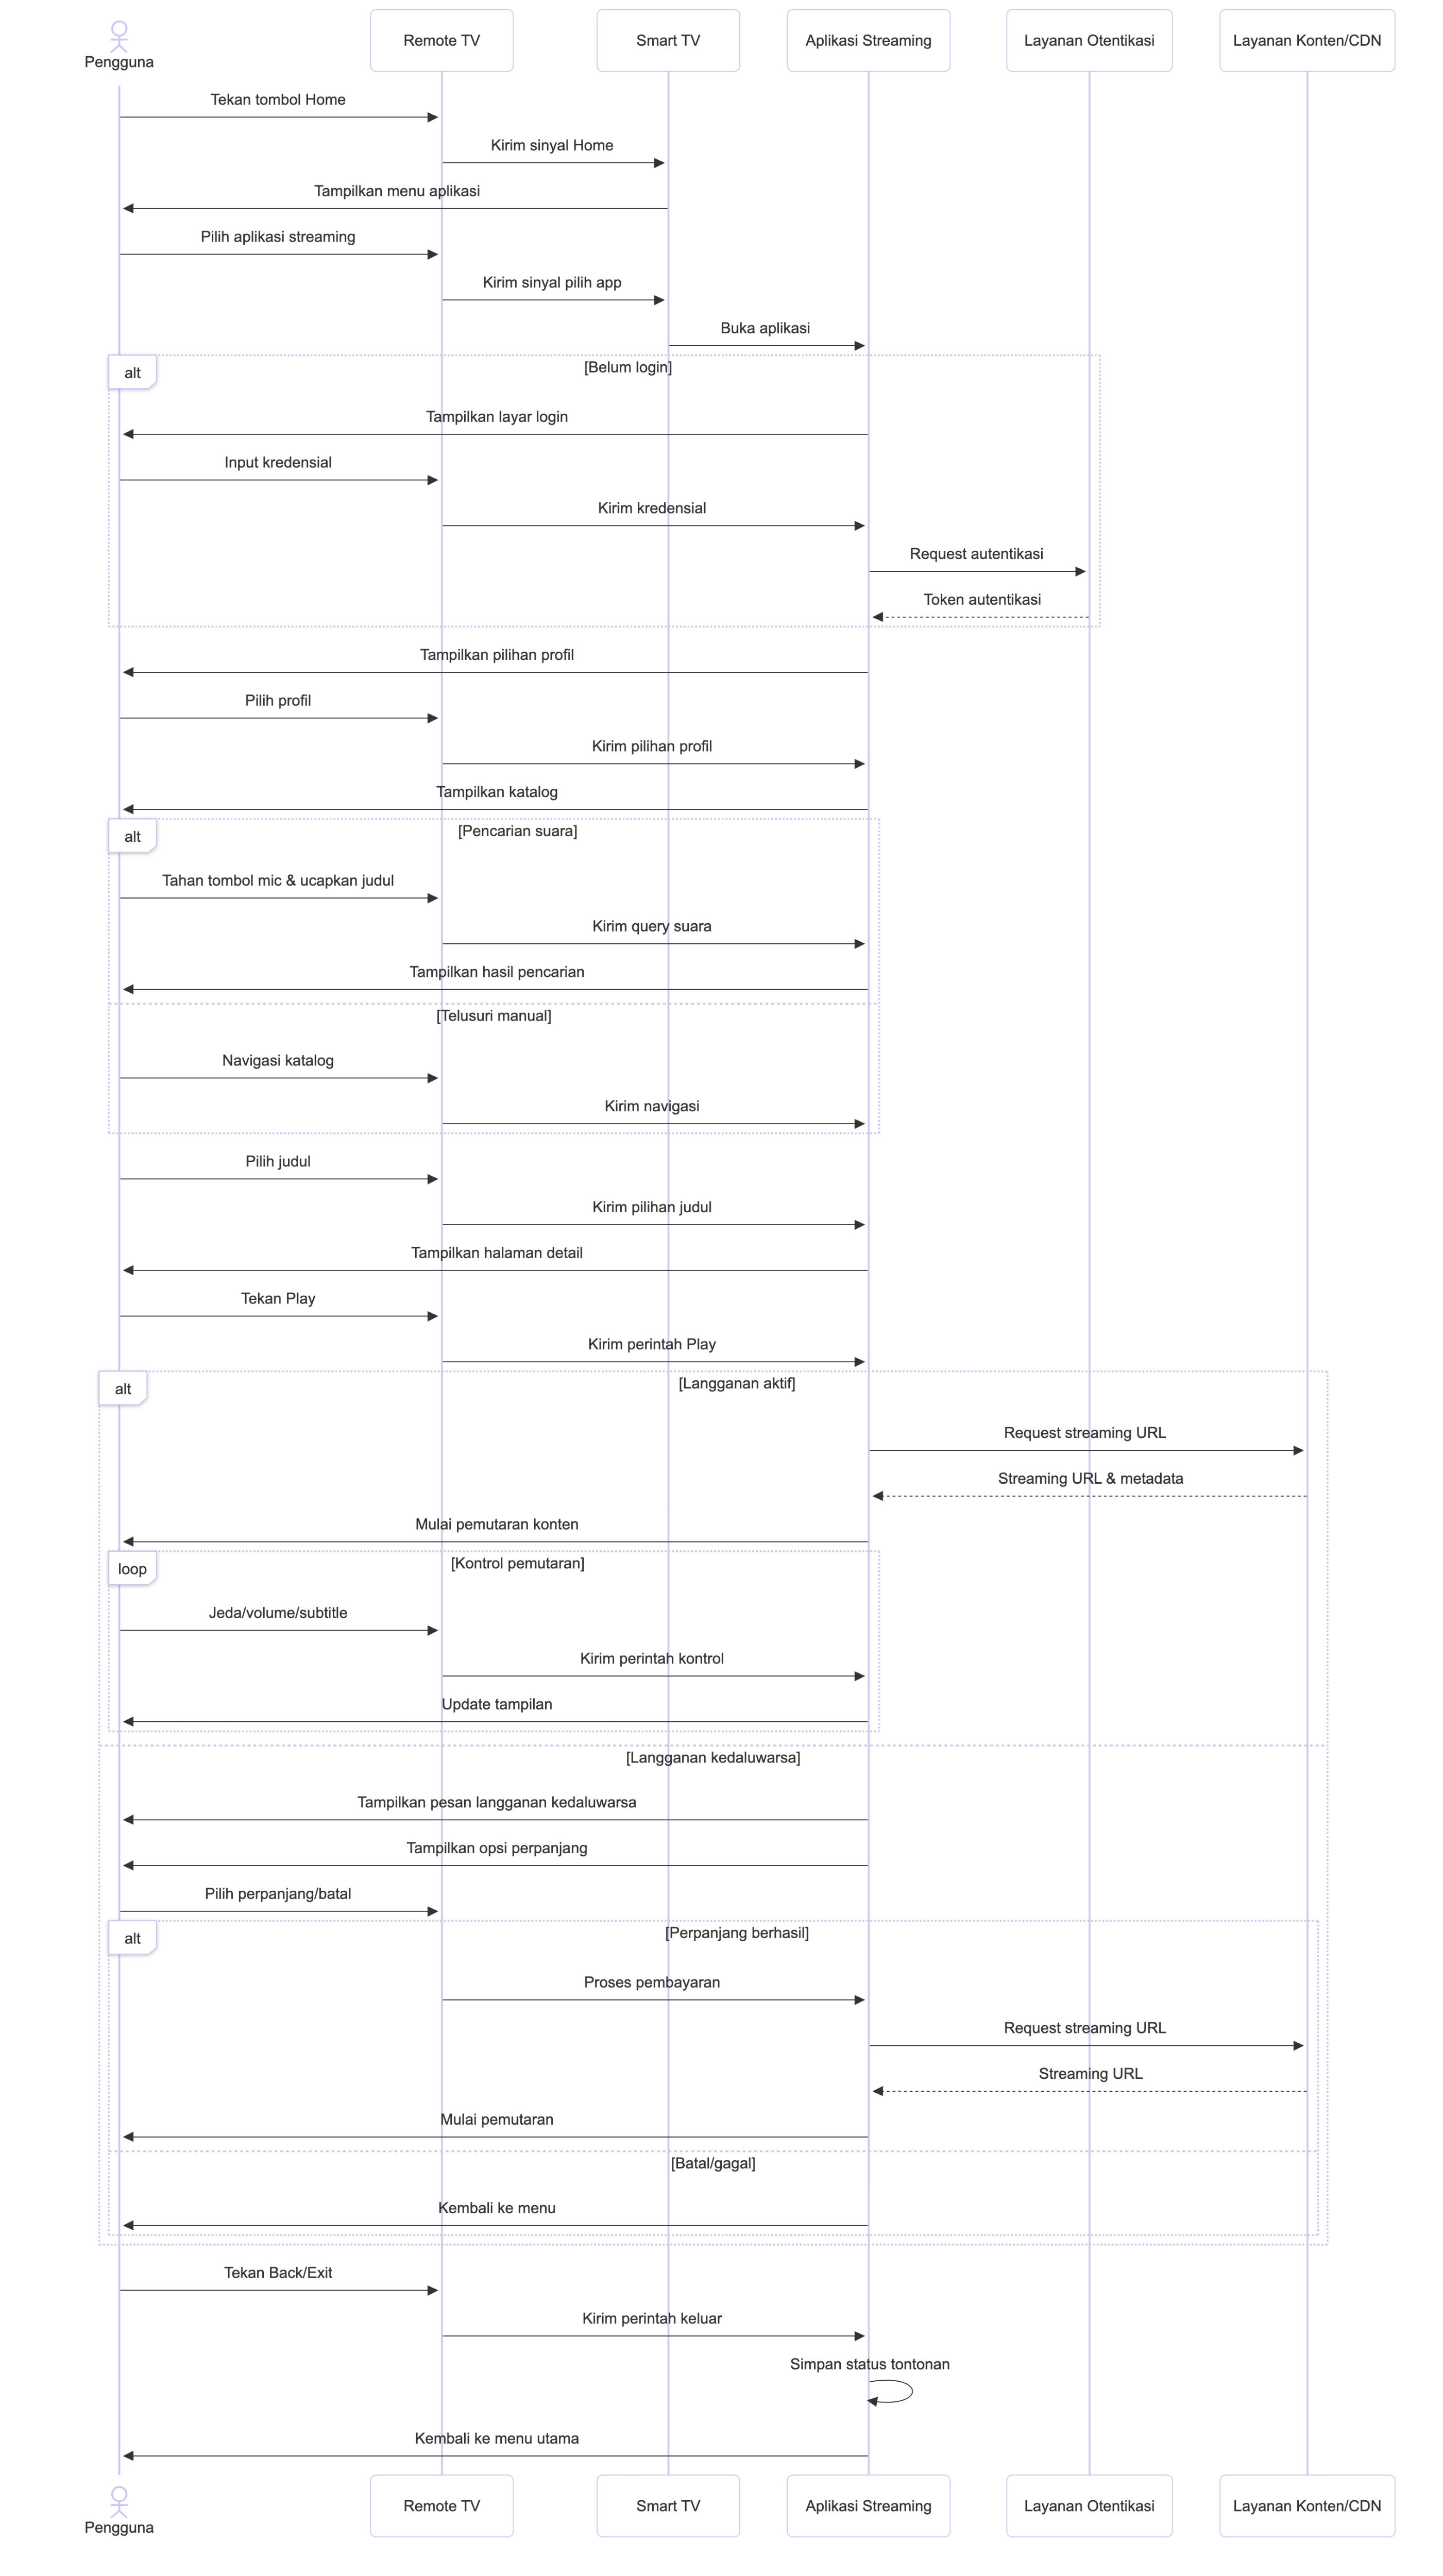
\includegraphics[height=0.9\textheight,keepaspectratio]{streaming-sequence-diagram.png}
    \end{center}
  \end{itemize}
  
  \pagebreak

  \begin{itemize}[itemsep=1em]
    \item Activity Diagram: Layanan Streaming dengan Remote TV
    \begin{center}
      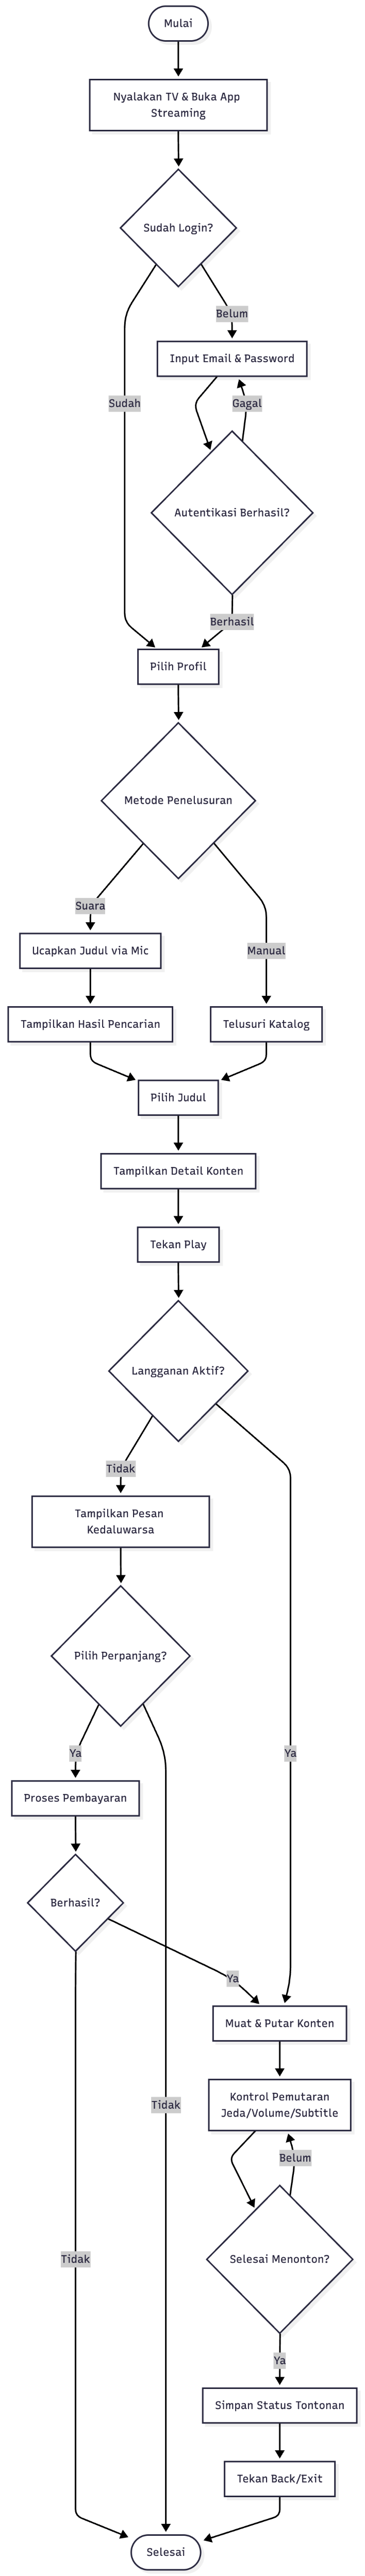
\includegraphics[height=0.9\textheight,keepaspectratio]{streaming-activity-diagram.png}
    \end{center}
  \end{itemize}
  
  \pagebreak

  \begin{itemize}[itemsep=1em]
    \item State Machine Diagram: Layanan Streaming dengan Remote TV
    \begin{center}
      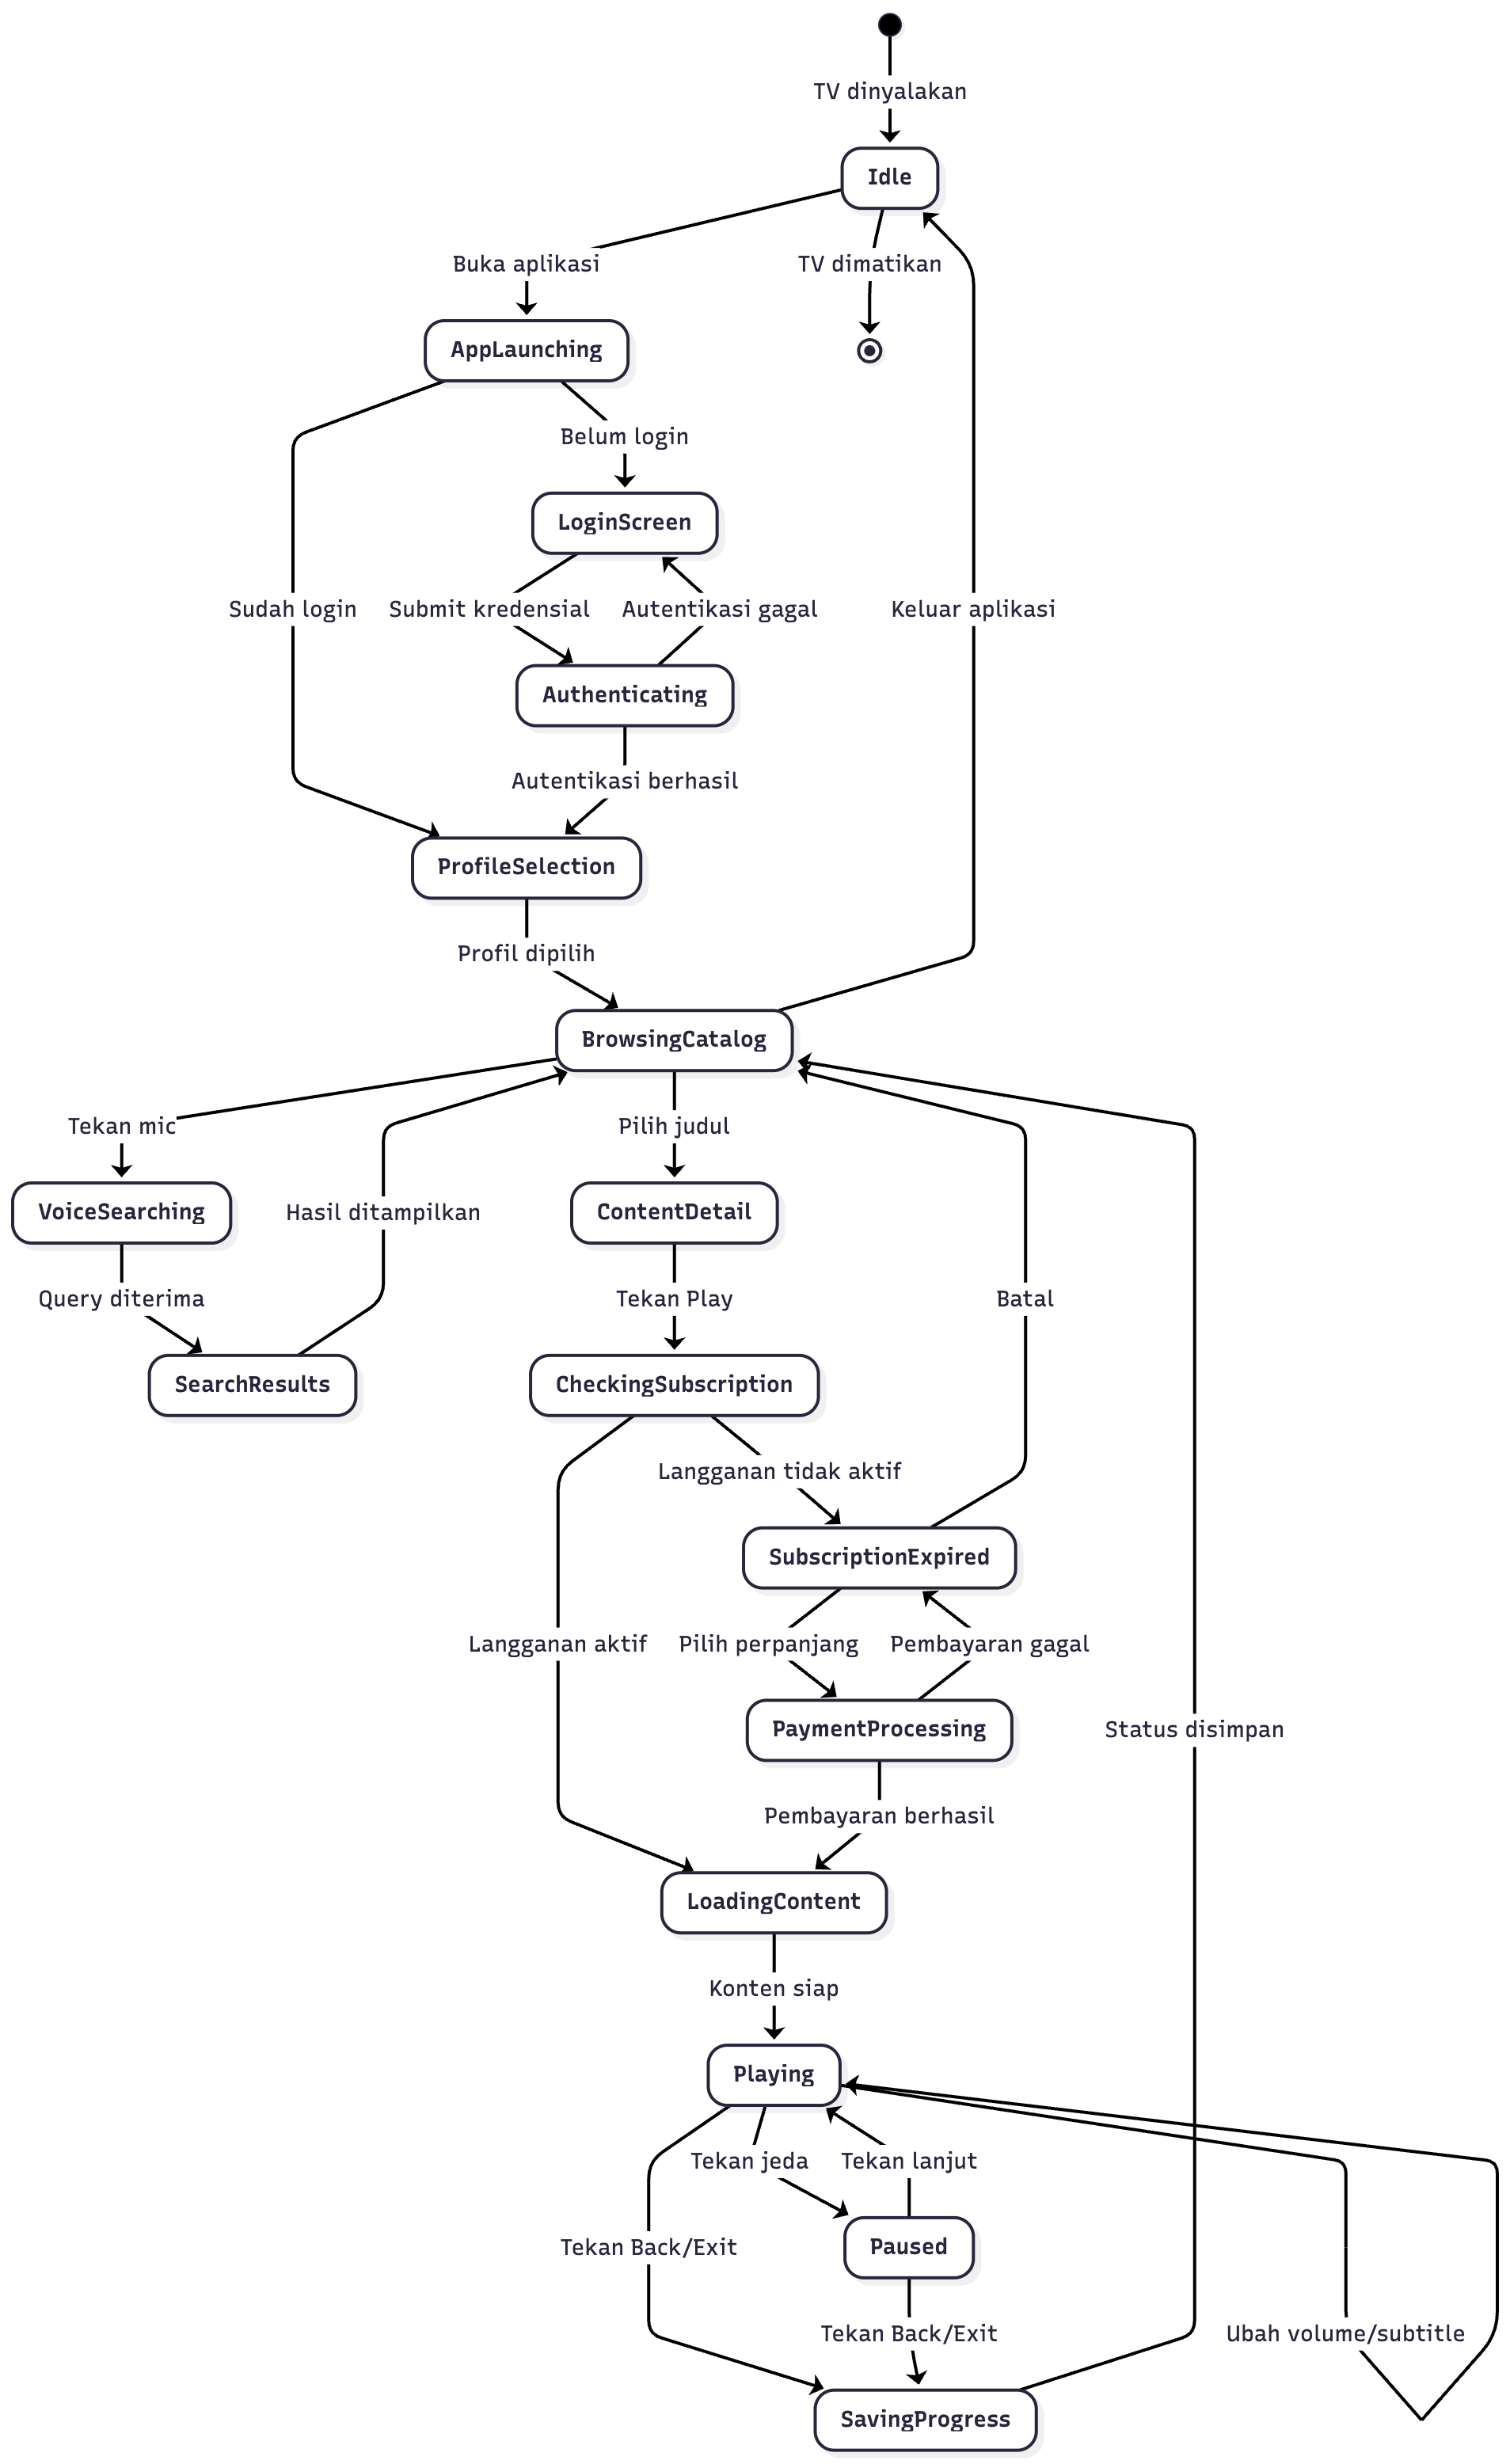
\includegraphics[width=0.65\textwidth,keepaspectratio]{streaming-state-diagram.png}
    \end{center}
  \end{itemize}

  \pagebreak

  \begin{itemize}[itemsep=1em]
    \item Sequence Diagram: Mengisi Tangki Bensin di Pom Bensin
    \begin{center}
      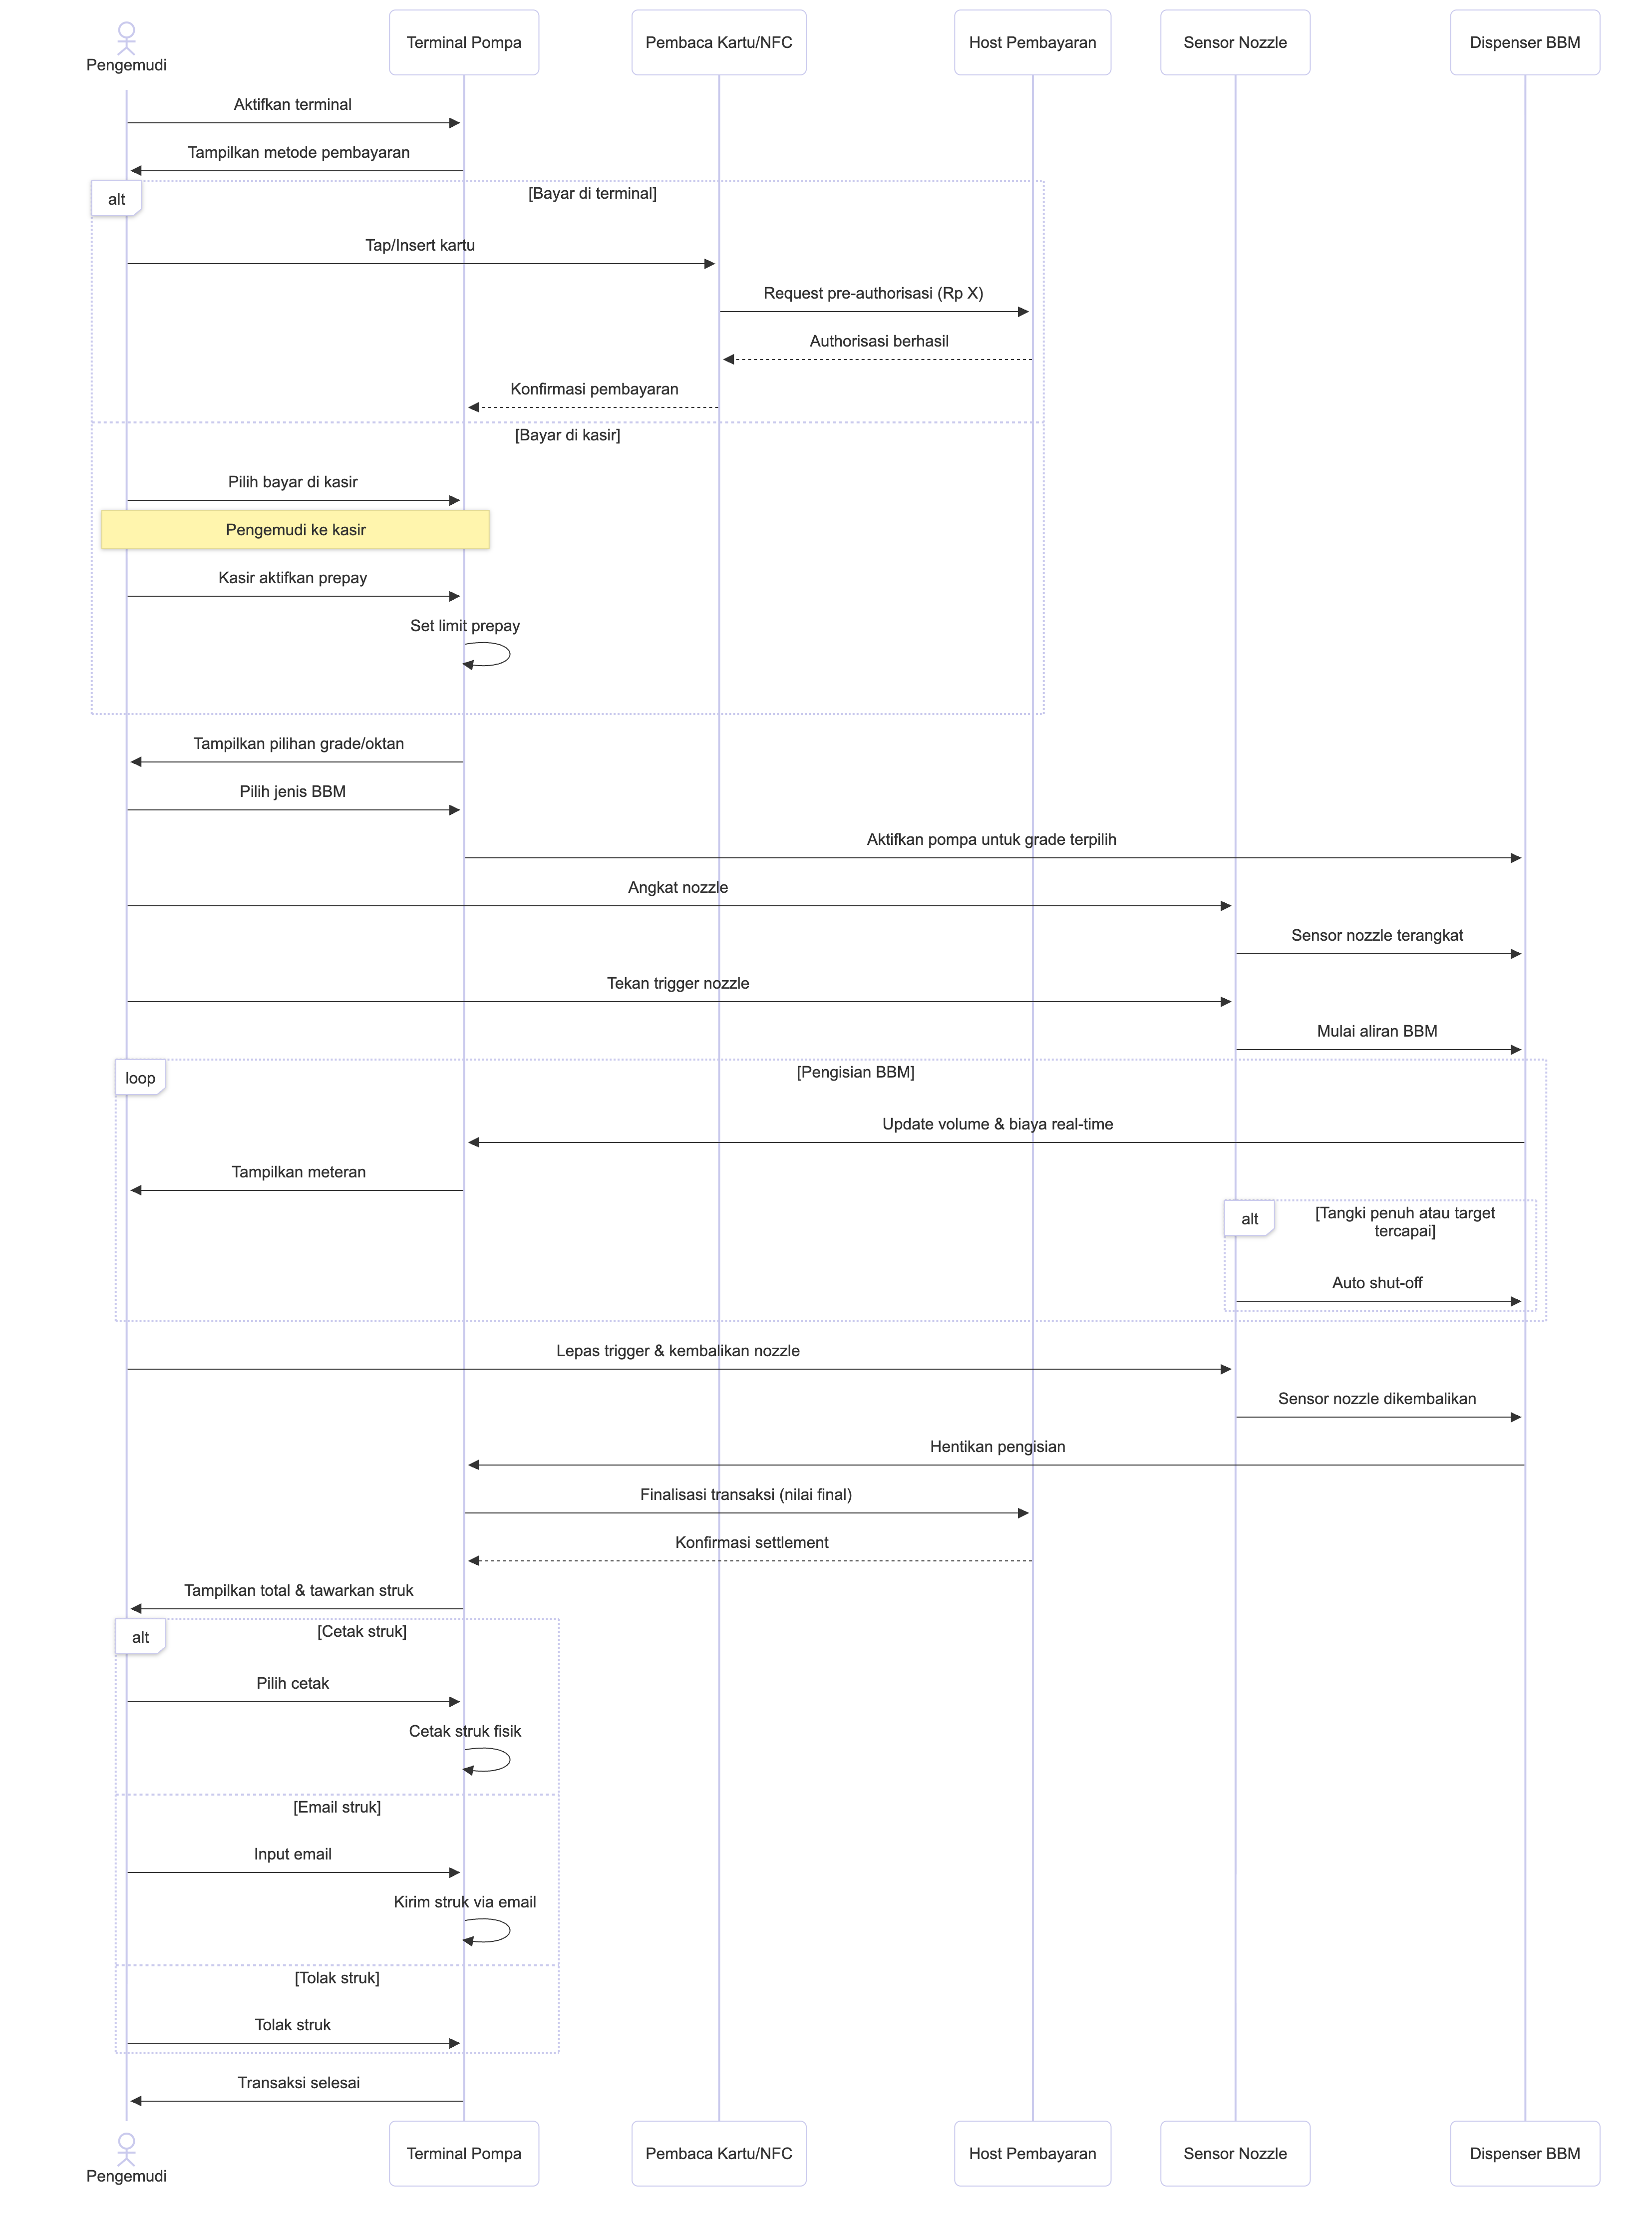
\includegraphics[width=0.9\textwidth,keepaspectratio]{fueling-sequence-diagram.png}
    \end{center}
  \end{itemize}

  \pagebreak

  \begin{itemize}[itemsep=1em]
    \item Activity Diagram: Mengisi Tangki Bensin di Pom Bensin
    \begin{center}
      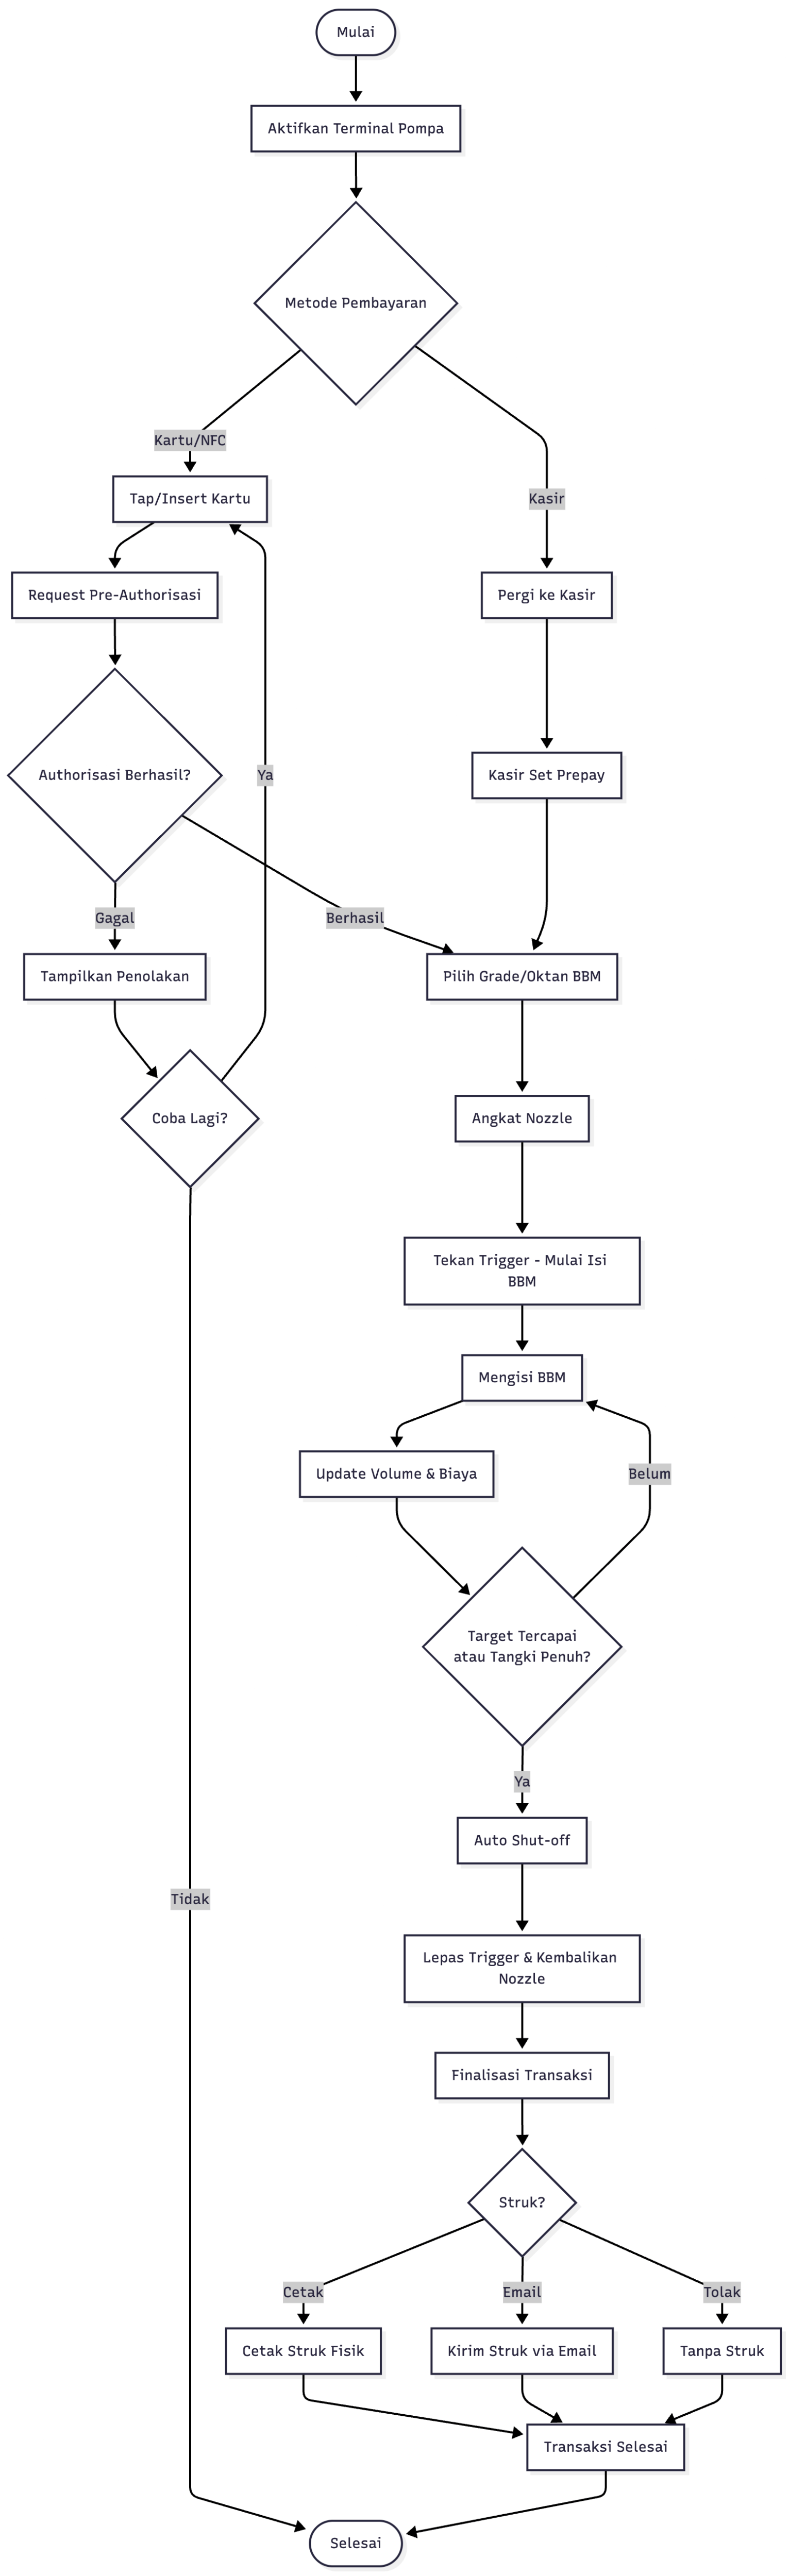
\includegraphics[height=0.9\textheight,keepaspectratio]{fueling-activity-diagram.png}
    \end{center}
  \end{itemize}

  \pagebreak

  \begin{itemize}[itemsep=1em]
    \item State Machine Diagram: Mengisi Tangki Bensin di Pom Bensin
    \begin{center}
      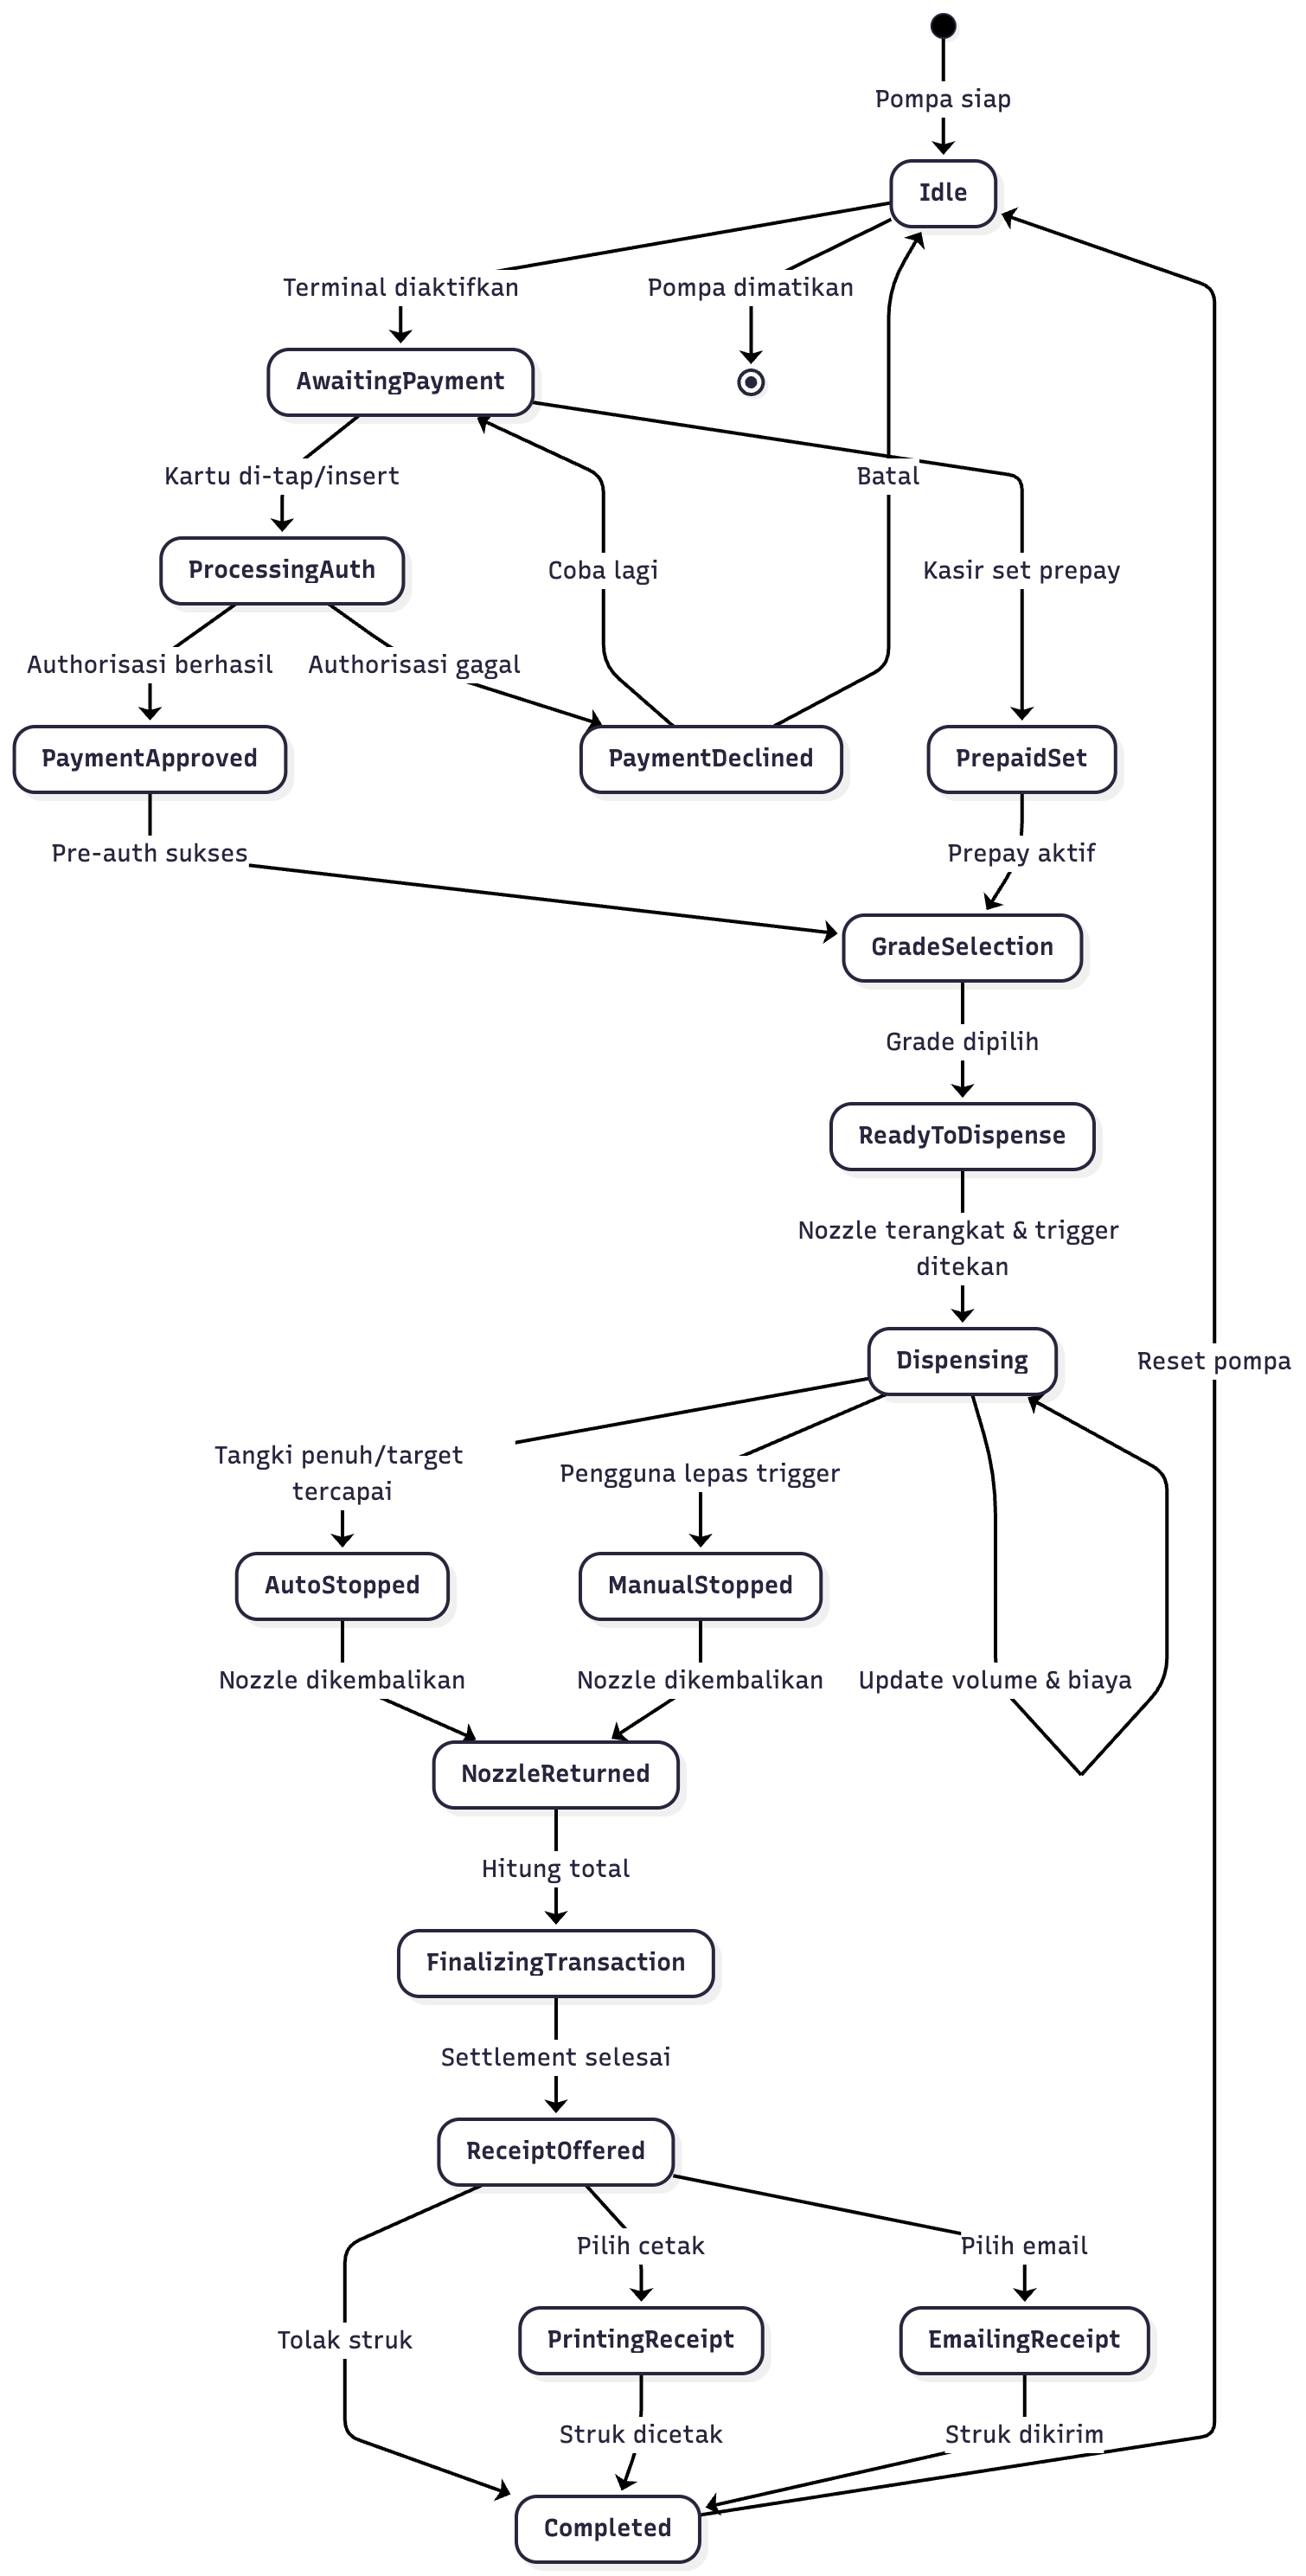
\includegraphics[width=0.65\textwidth,keepaspectratio]{fueling-state-diagram.png}
    \end{center}
  \end{itemize}

  \pagebreak

  \begin{itemize}[itemsep=1em]
    \item Sequence Diagram: Pembayaran Mandiri di Toko Kelontong
    \begin{center}
      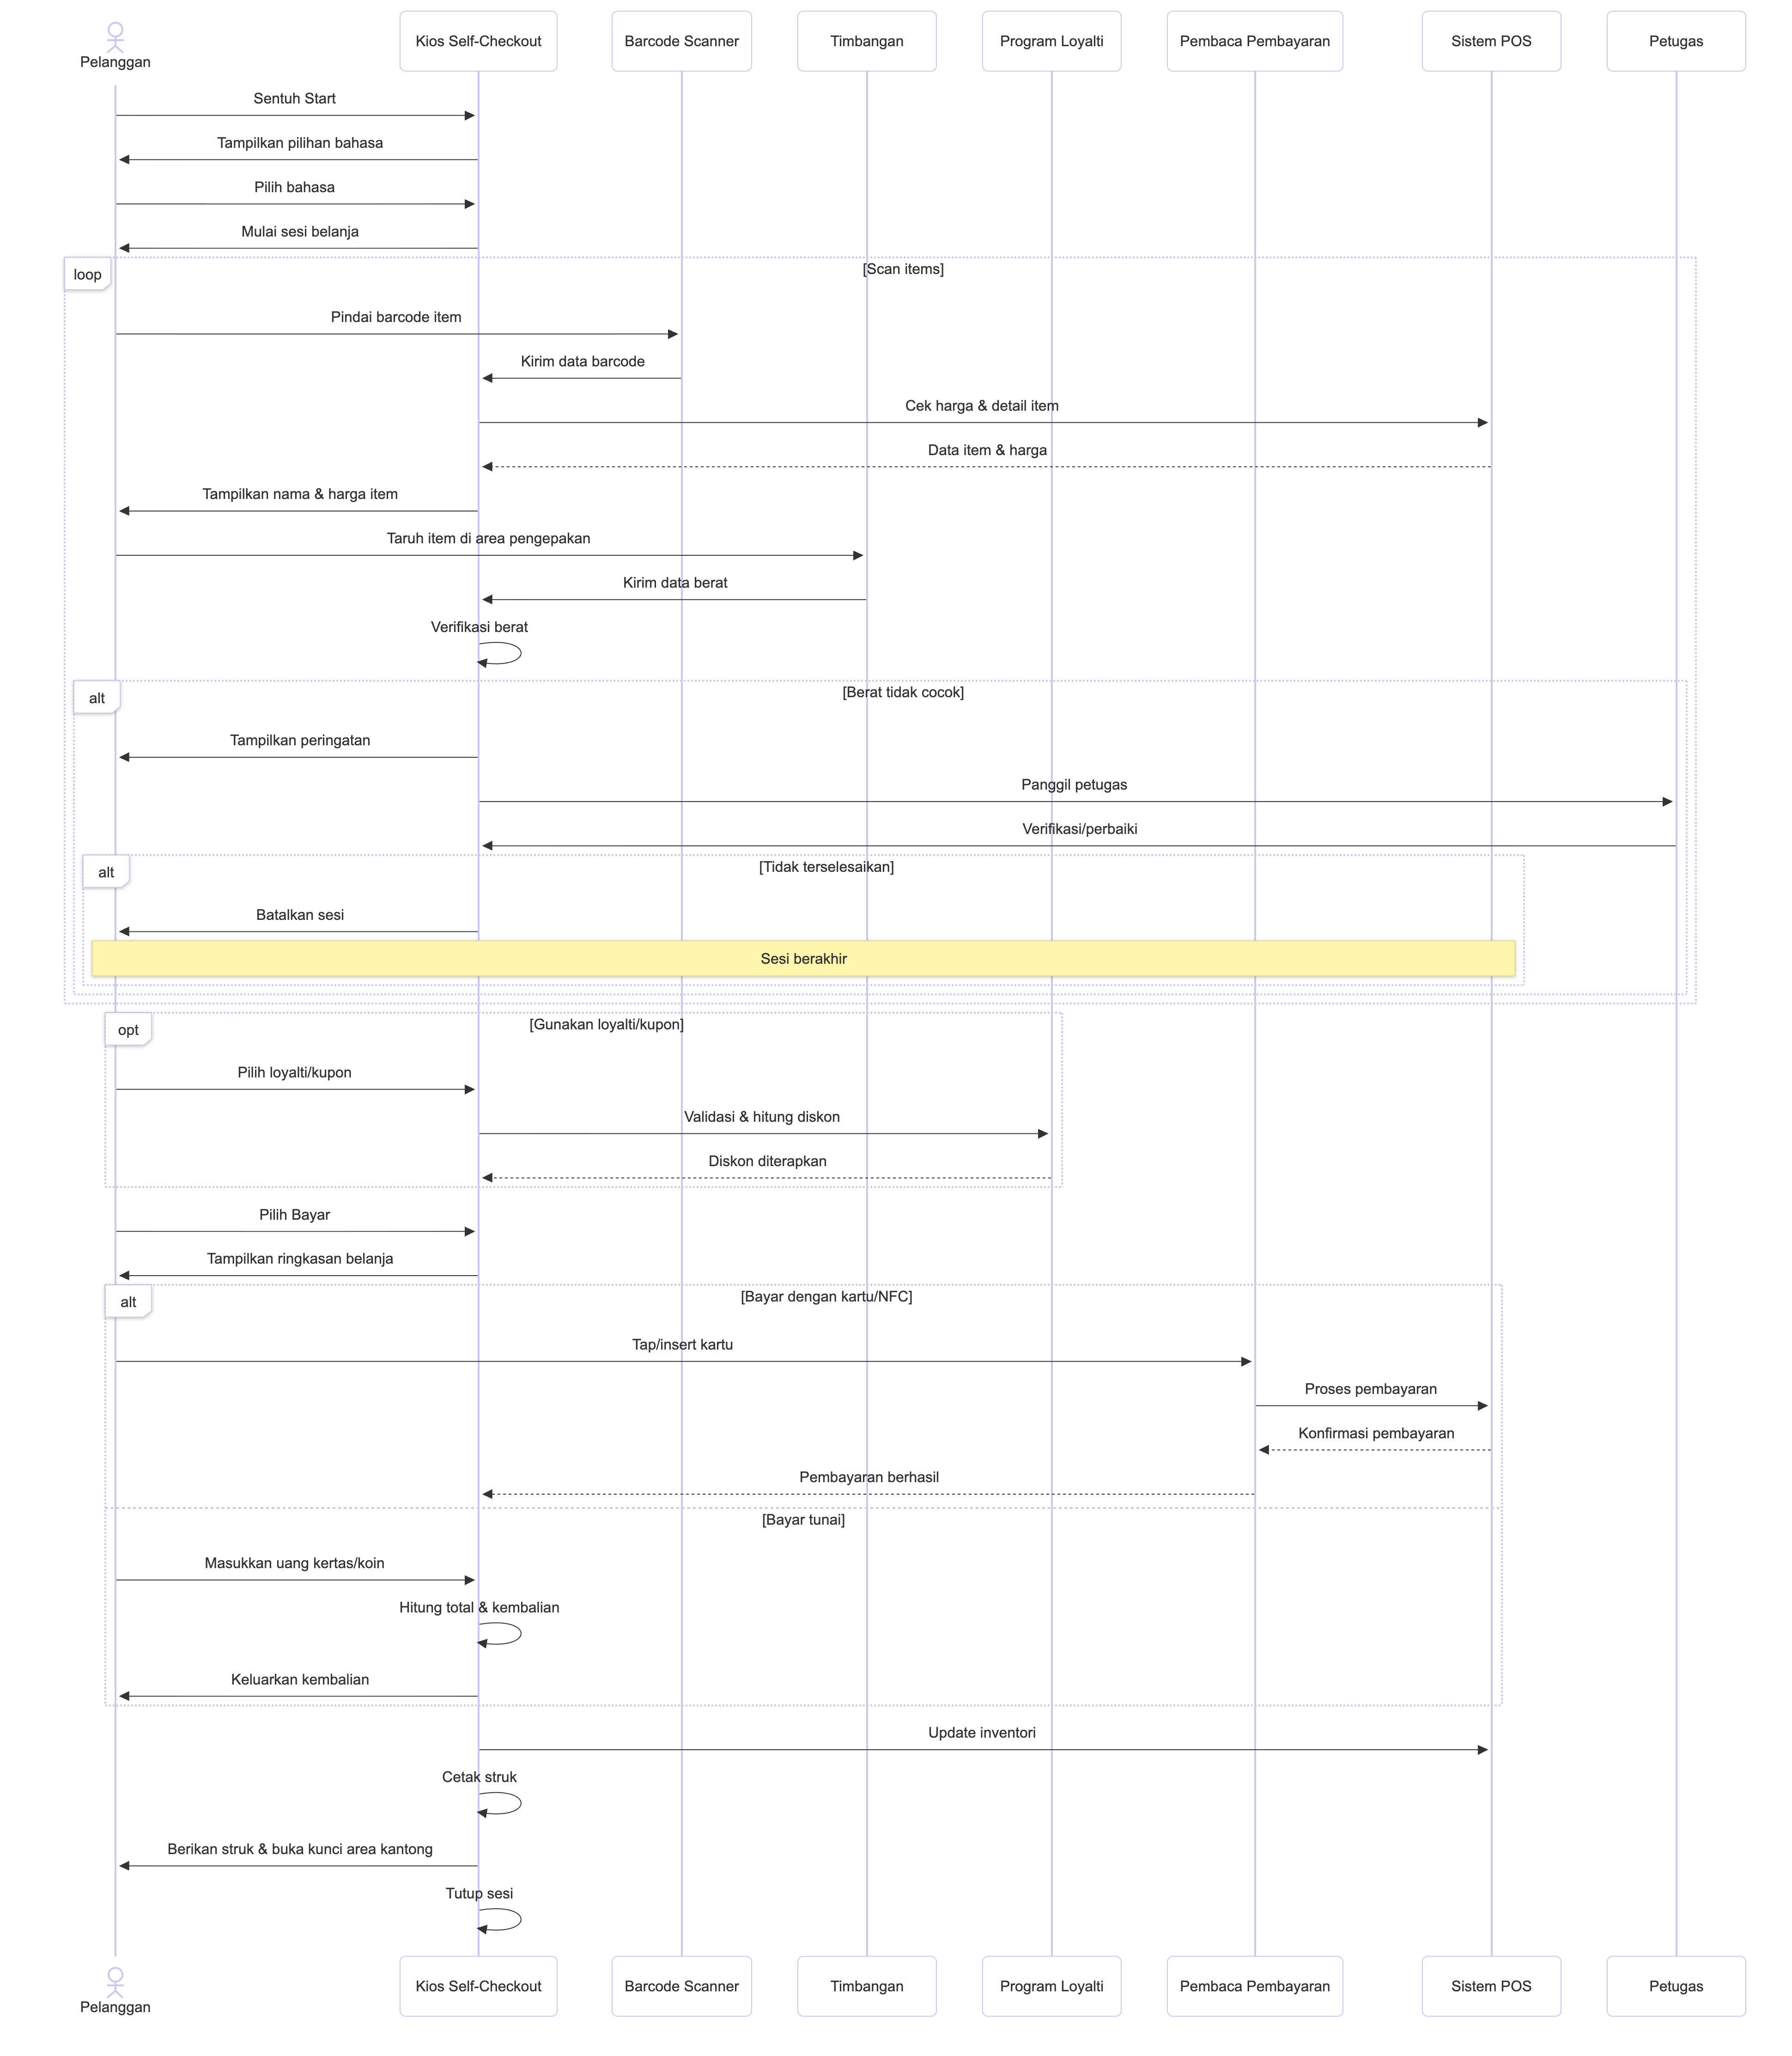
\includegraphics[width=0.85\textwidth,keepaspectratio]{self-checkout-sequence-diagram.png}
    \end{center}
  \end{itemize}

  \pagebreak

  \begin{itemize}[itemsep=1em]
    \item Activity Diagram: Pembayaran Mandiri di Toko Kelontong
    \begin{center}
      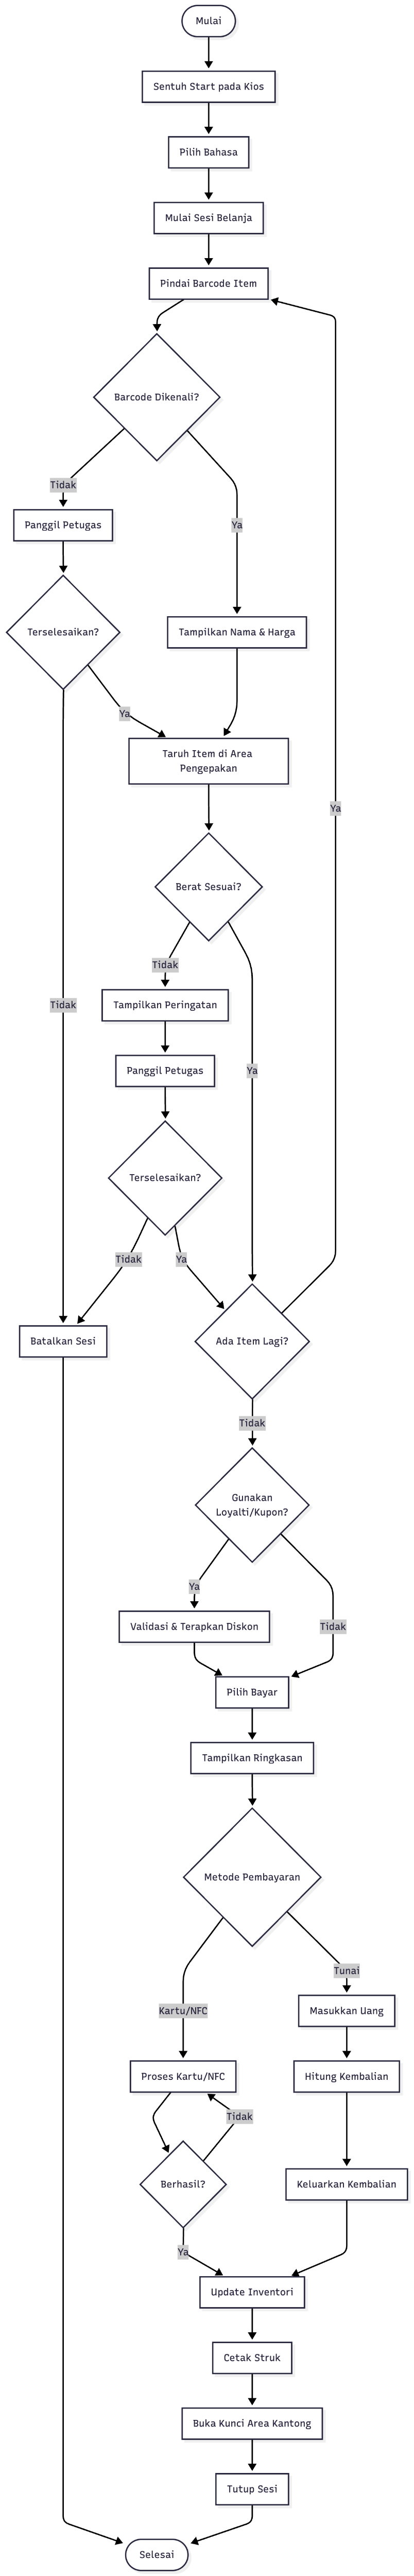
\includegraphics[height=0.9\textheight,keepaspectratio]{self-checkout-activity-diagram.png}
    \end{center}
  \end{itemize}

  \pagebreak

  \begin{itemize}[itemsep=1em]
    \item State Machine Diagram: Pembayaran Mandiri di Toko Kelontong
    \begin{center}
      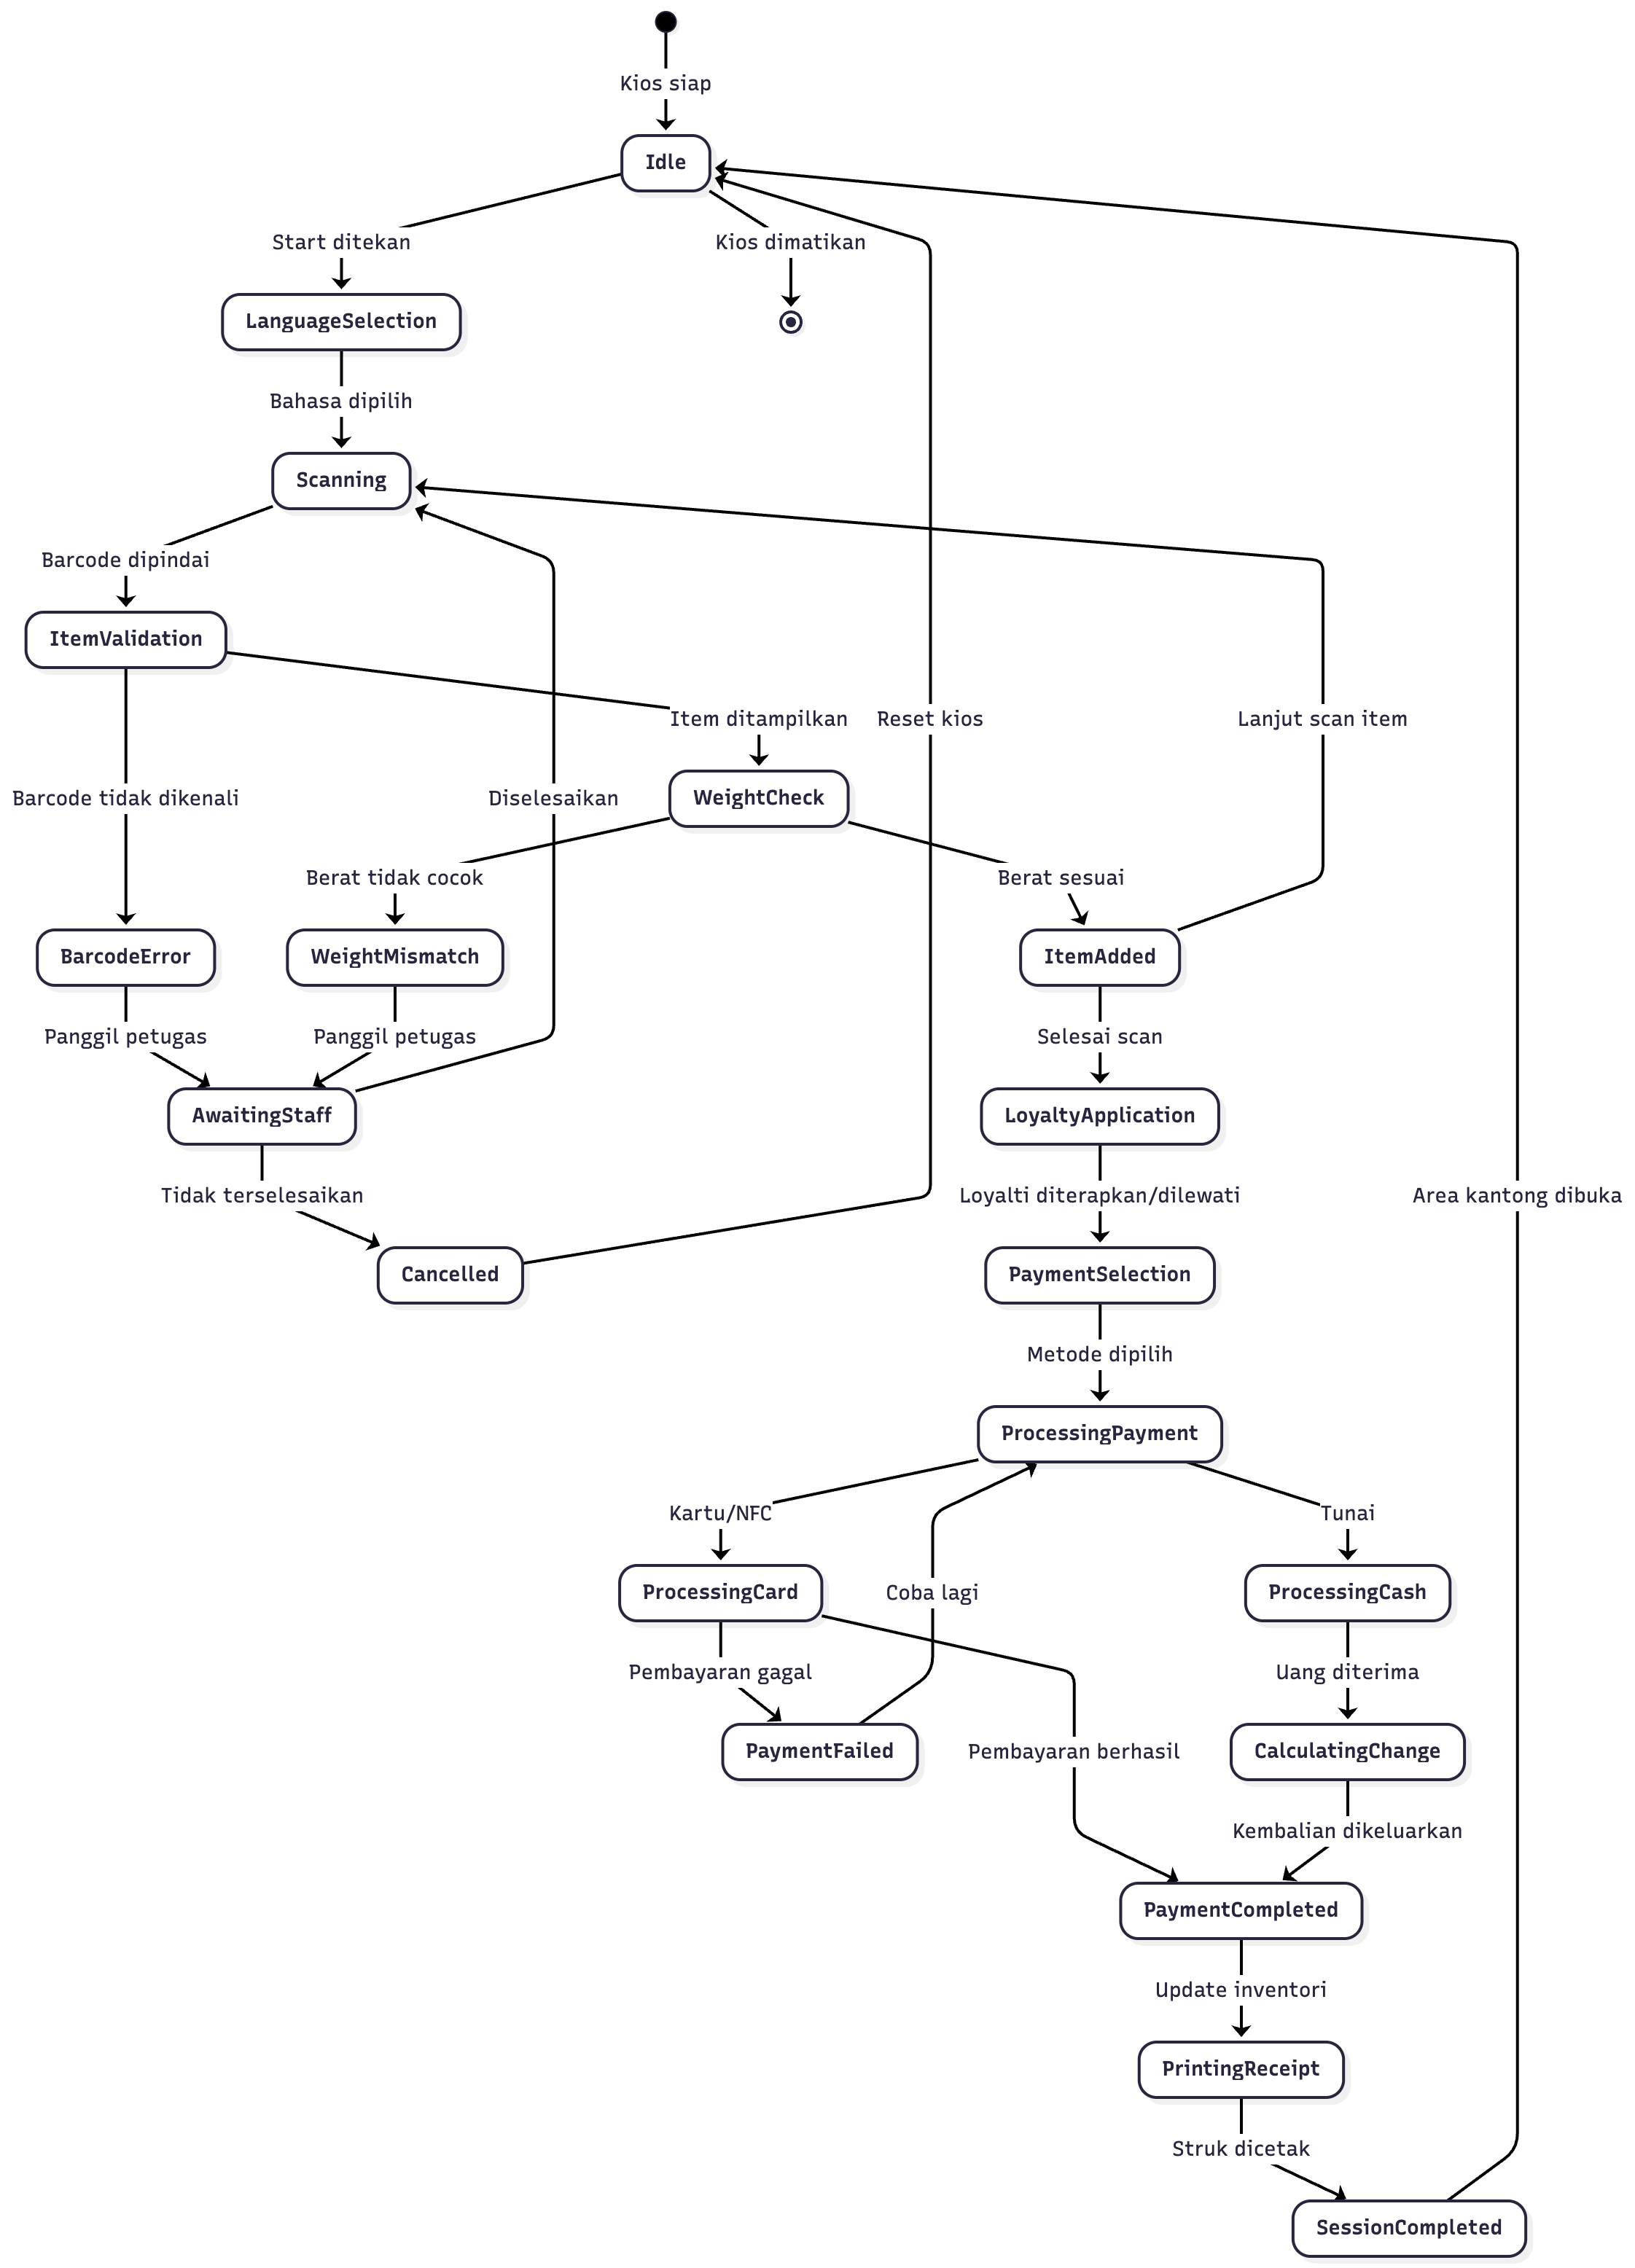
\includegraphics[width=0.65\textwidth,keepaspectratio]{self-checkout-state-diagram.png}
    \end{center}
  \end{itemize}
  
  \pagebreak
  
  \begin{itemize}[itemsep=1em]
    \item Sequence Diagram: Pembayaran Mandiri di Bandara
    \begin{center}
      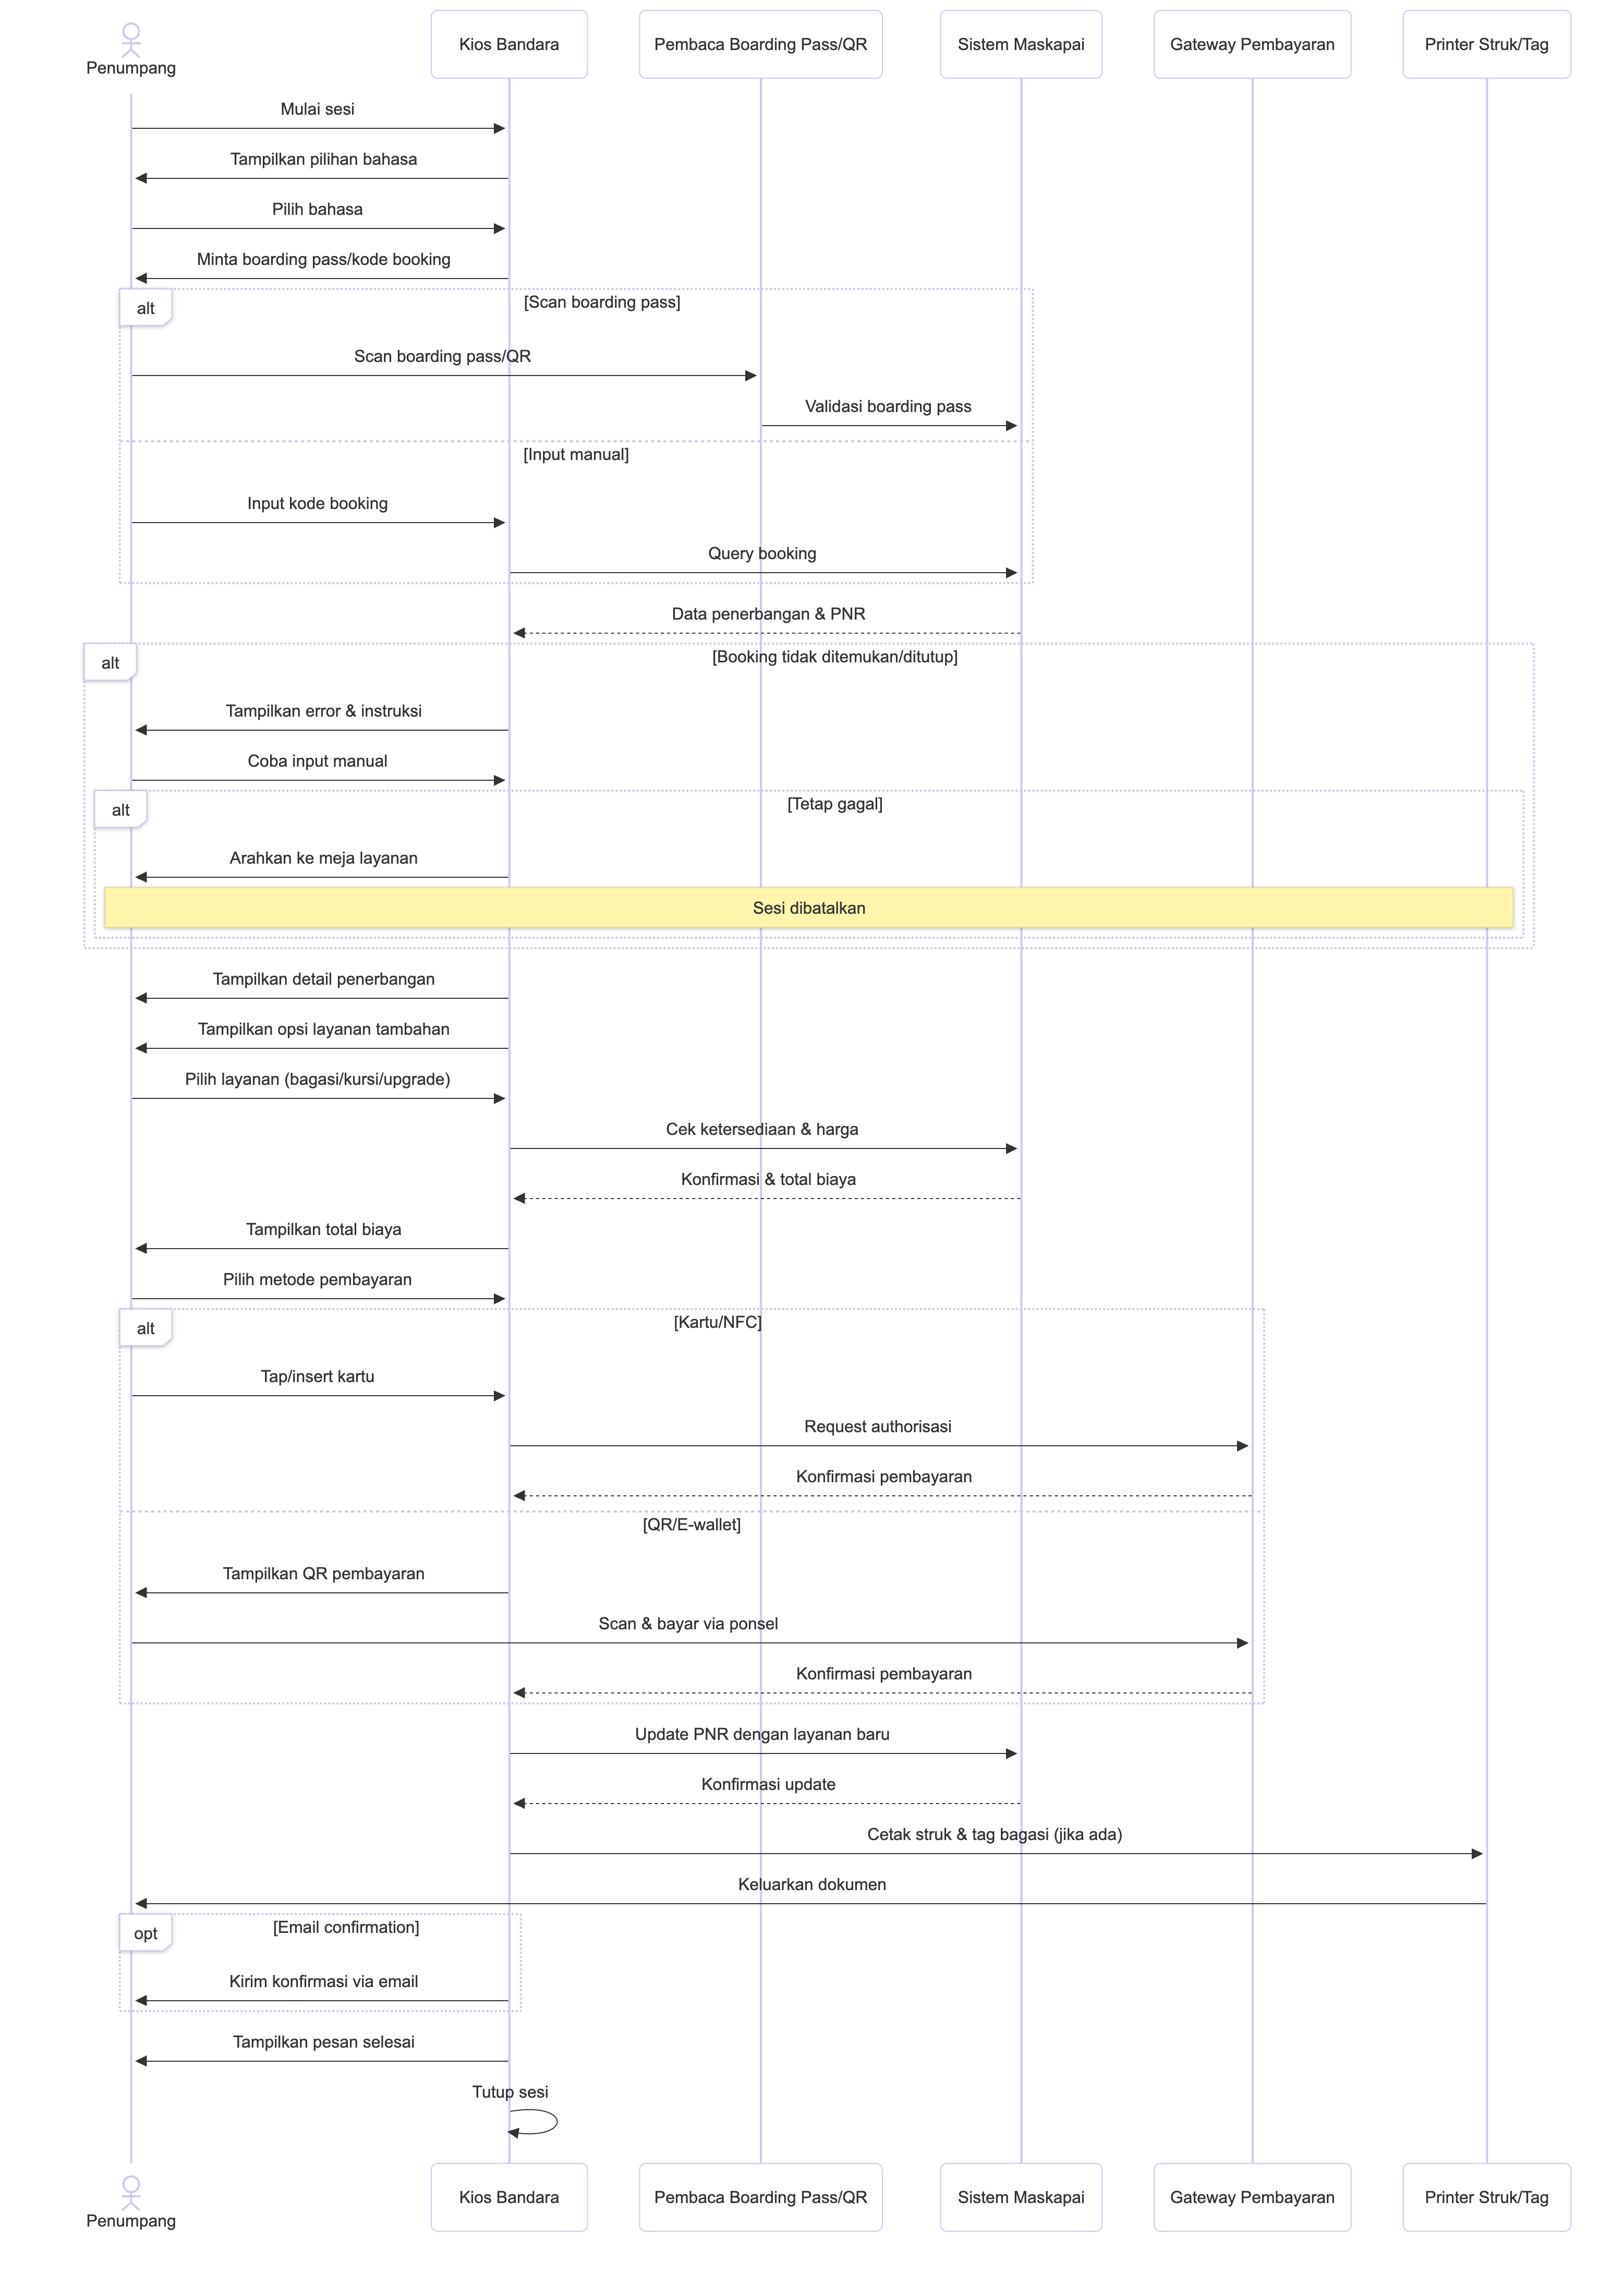
\includegraphics[width=0.85\textwidth,keepaspectratio]{airport-payment-sequence-diagram.png}
    \end{center}
  \end{itemize}
  
  \pagebreak

  \begin{itemize}[itemsep=1em]
    \item Activity Diagram: Pembayaran Mandiri di Bandara
    \begin{center}
      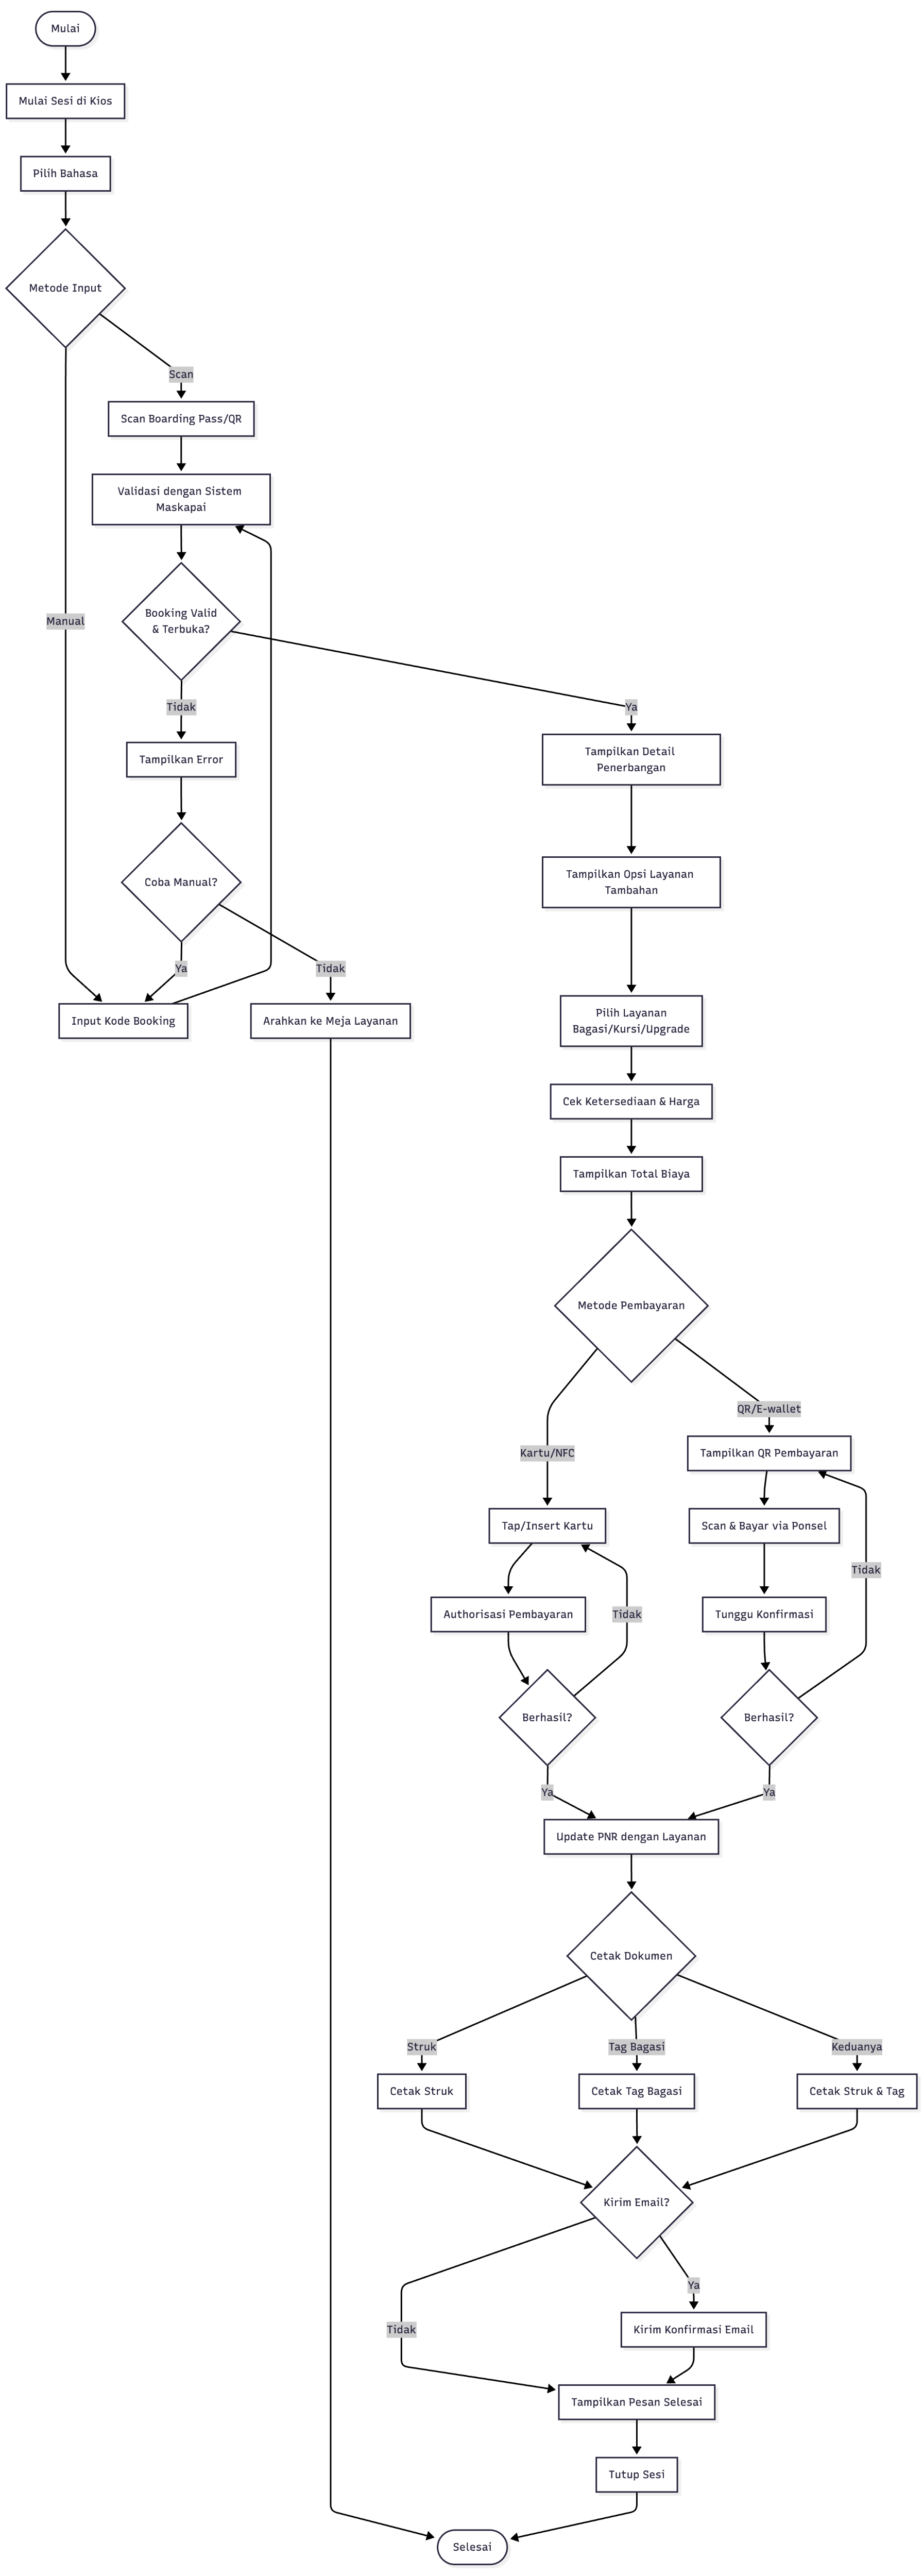
\includegraphics[height=0.9\textheight,keepaspectratio]{airport-payment-activity-diagram.png}
    \end{center}
  \end{itemize}
  
  \pagebreak

  \begin{itemize}[itemsep=1em]
    \item State Machine Diagram: Pembayaran Mandiri di Bandara
    \begin{center}
      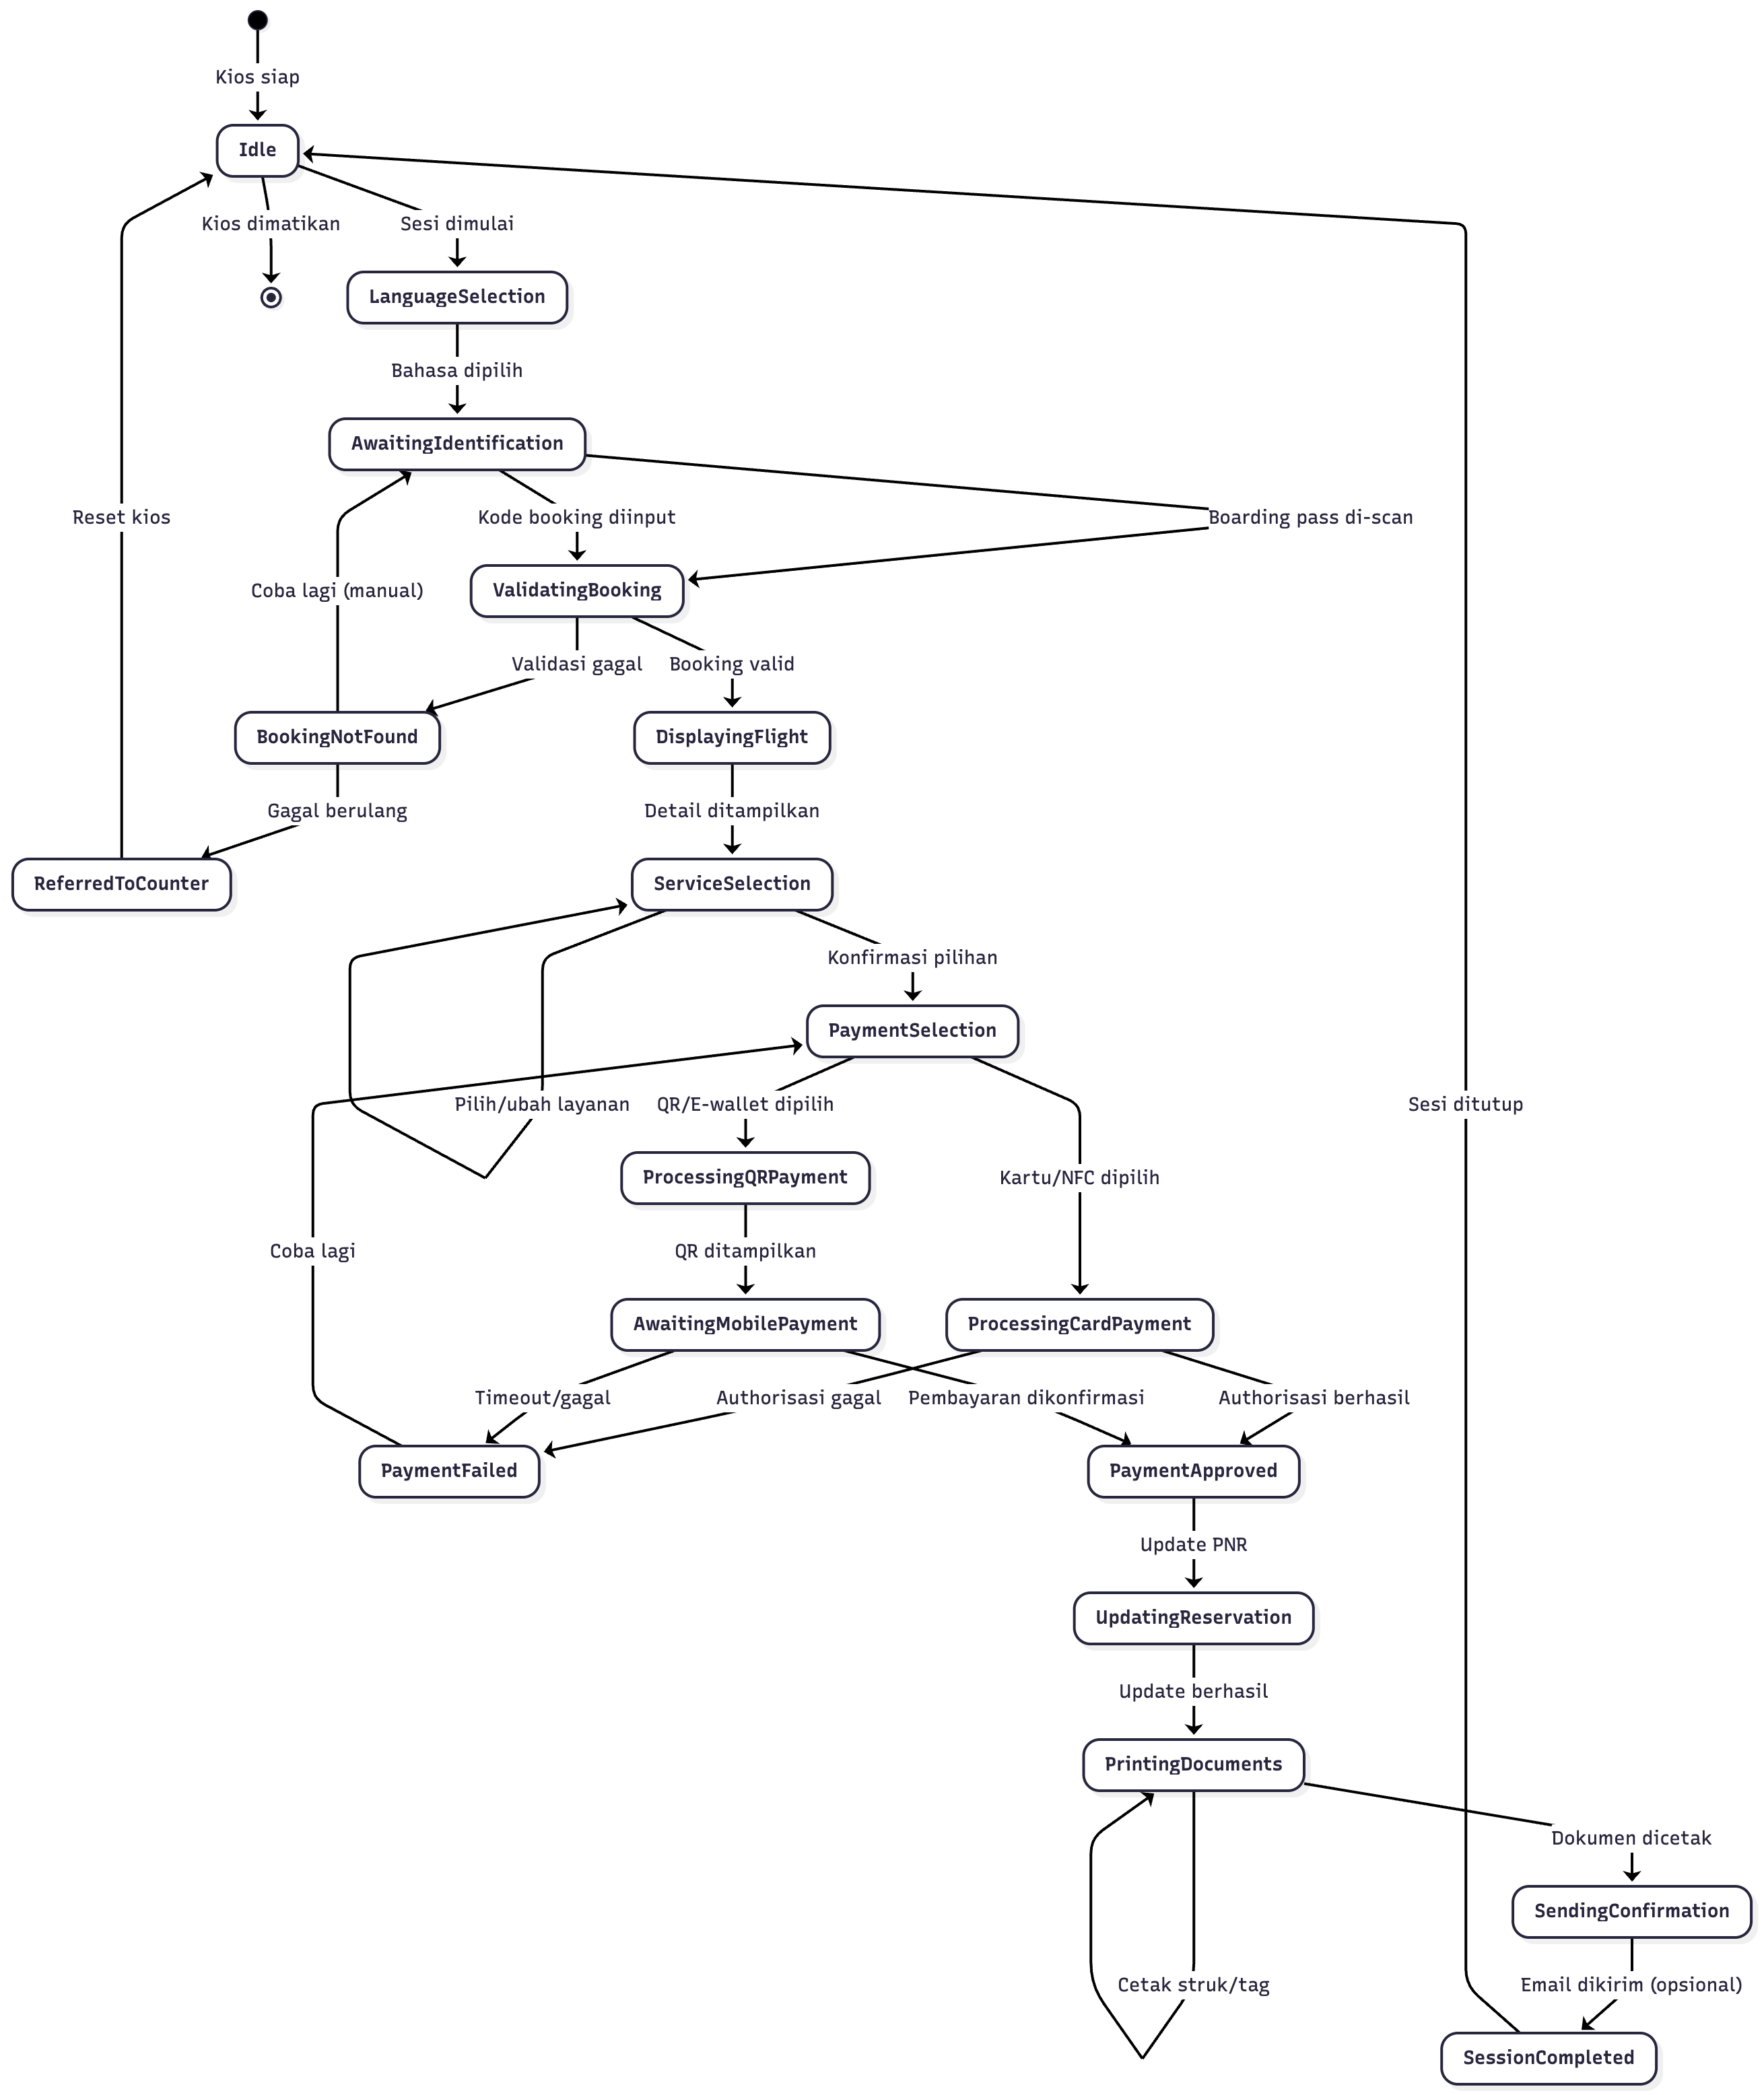
\includegraphics[width=0.65\textwidth,keepaspectratio]{airport-payment-state-diagram.png}
    \end{center}
  \end{itemize}

  \vspace{1em}

  \item (LO 3: 25\%) (LN 08 topik - Software Design Patterns)

  Gunakan pola Abstract Factory untuk membuat pabrik dengan dua produk tombol: satu yang mengubah warna latar belakang tombol saat mouse diarahkan dan yang lainnya yang mengubah dua warna latar belakang saat diklik.

  \item (LO 3: 50\%) (LN 09 topik - Software Architecture and Architecture Views; LN 05 topik - Design case studies)
  
  Asumsikan Anda ingin menulis program Java yang menganimasikan bola yang bergerak bebas dan terpantul saat mengenai tepi (lalu bergerak ke arah pantulan). Bola dimanipulasi dengan utas terpisah.

  \vspace{1em}

  Berikan tampilan logika dari Model Tampilan 4+1 yang berfokus pada cara kerja program pada tingkat tinggi dan tampilan proses yang berfokus pada cara thread bola berinteraksi dengan thread utama.
\end{enumerate}

Referensi:

\begin{itemize}
  \item Lecture Note 5.
  \item Lecture Note 6.
  \item Lecture Note 7.
  \item Lecture Note 8.
  \item Lecture Note 9.
\end{itemize}

\end{document}
